% Created 2018-06-27 Wed 19:10
%updated 2020-09-29 _Imam Al Razi
\documentclass[11pt]{article}
\usepackage[utf8]{inputenc}
\usepackage[T1]{fontenc}
\usepackage{fixltx2e}
\usepackage{graphicx}
\usepackage{subfig}
\usepackage{longtable}
\usepackage{float}
\usepackage{wrapfig}
\usepackage{rotating}
\usepackage[normalem]{ulem}
\usepackage{amsmath}
\usepackage{textcomp}
\usepackage{marvosym}
\usepackage{wasysym}
\usepackage{amssymb}
\usepackage{hyperref}
\usepackage{listings}
\setlength{\tabcolsep}{4pt}

\DeclareMathOperator{\HYPHEN}{-}


\newcommand{\bigstrut}[1][]{}

\lstset{
basicstyle=\ttfamily,
frame = single, 
framexleftmargin=15pt}
\tolerance=1000
\usepackage[margin=2.5cm]{geometry}
\renewcommand\maketitle{}
\usepackage[style=ieee]{biblatex}
\date{\today}
\title{PowerSynth User Manual Version 1.9}

\hypersetup{
  pdfkeywords={},
  pdfsubject={},
  pdfcreator={Emacs 25.2.1 (Org mode 8.2.10)}}
\begin{document}

\maketitle
\begin{titlepage}
\begin{center}

\begin{figure}[h!]
  \centering
  
\includegraphics[width=0.4\linewidth]{./figs/00_UarkLogo.eps}
\end{figure}

{\Large Mixed-Signal Computer-Aided Deisgn \href{https://mscad.uark.edu/}{(\underline{$MSCAD$})}  Laboratory \par}
{\Large Energy-Efficient Electronics and Design Automation \href{https://e3da.csce.uark.edu/}{(\underline{$E^3DA$})} Laboratory \par}
\vspace{2cm}
{\Huge PowerSynth User Manual\\ Version 1.9 \par}
\vspace{1cm}

\vspace{1cm}

\begin{figure}[h!]
  \centering
  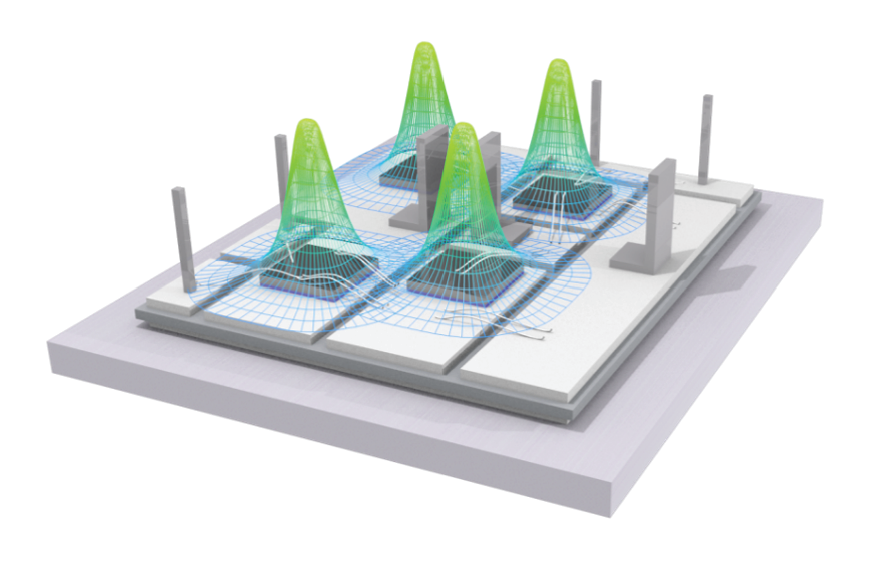
\includegraphics[width=\linewidth]{./figs/00_PS.eps}
\end{figure}

\end{center}
\end{titlepage}





\tableofcontents
\pagebreak

\section{Introduction}
\label{sec-1}

\subsection{Executive Summary}
\label{sec-1-1}
\subsubsection{PowerSynth Introduction}
PowerSynth is an electronic design automation (EDA) tool that can synthesize and optimize multi-chip power module (MCPM) layouts with significantly faster than any commercial tools. PowerSynth currently performs multi-objective optimization to produce Pareto-front solutions to the proper placement of power semiconductor device die and the routing of metal traces on ceramic substrates. The tool accounts for temperature distributions and electrical parasitics as a function of the layout geometries that it considers. This tool has been hardware-validated. Continued research on this project will further elaborate the capabilities by extending the work to greater fidelity in thermal, electrical, and mechanical domains.

\subsubsection{About Version 1.9}
As a part of PowerSynth continuous research and development, this version (v1.9) offers a command line interface to the users with a significant improvement in layout representation and generation methodology. 
Some of the major features in this version include:
\begin{itemize}
\item Generic layout representation technique for complex (2D/2.5D) geometry handling.
\item Hierarchical constraint-aware, generic, efficient, and scalable layout generation methodology.
\item Heretogeneous components handling.
\item Rigid and flexible bonding wire connections.
\item Voltage-current dependent reliability constraints handling.
\item Arbitrary number of passive layers in the layer stack.
\item Initial(single) layout performance evaluation.
\item Partial element equivalent circuit (PEEC) based electrical model.
\item Hardware-validated, fast, and accurate thermal model.
\end{itemize} 
It is recommended that the user reads the manual of the previous version (v1.4) to have a better understanding of the feature-wise differences in between this and the old version. The previous versions of PowerSynth had graphical user interface (GUI) and some features like 3D solution browser, export to 3D modeling and FEA tools, and these features will be added back in our upcoming release (v2.0) with 3D MCPM layout optimization capability.
\subsection{Organization}
\label{sec-1-2}
After a brief introduction to PowerSynth v1.9 architecture, this document introduces the command line workflow. This document will show the user how to prepare the necessary files, and parameters for using this version. Then, this document walks the user through the steps to optimize a sample 2D half-bridge power module.

\subsection{PowerSynth v1.9 Architecture}
\label{sec-1-3}
Since the very first version of PowerSynth (v1.0), some new models are developed to incorporate new objectives for optimization, and some features have been added to add more capabilities over time. The latest architecture in v1.9 release is shown in Figure~\ref{fig:architecture}.


\begin{figure}[t]
\centering
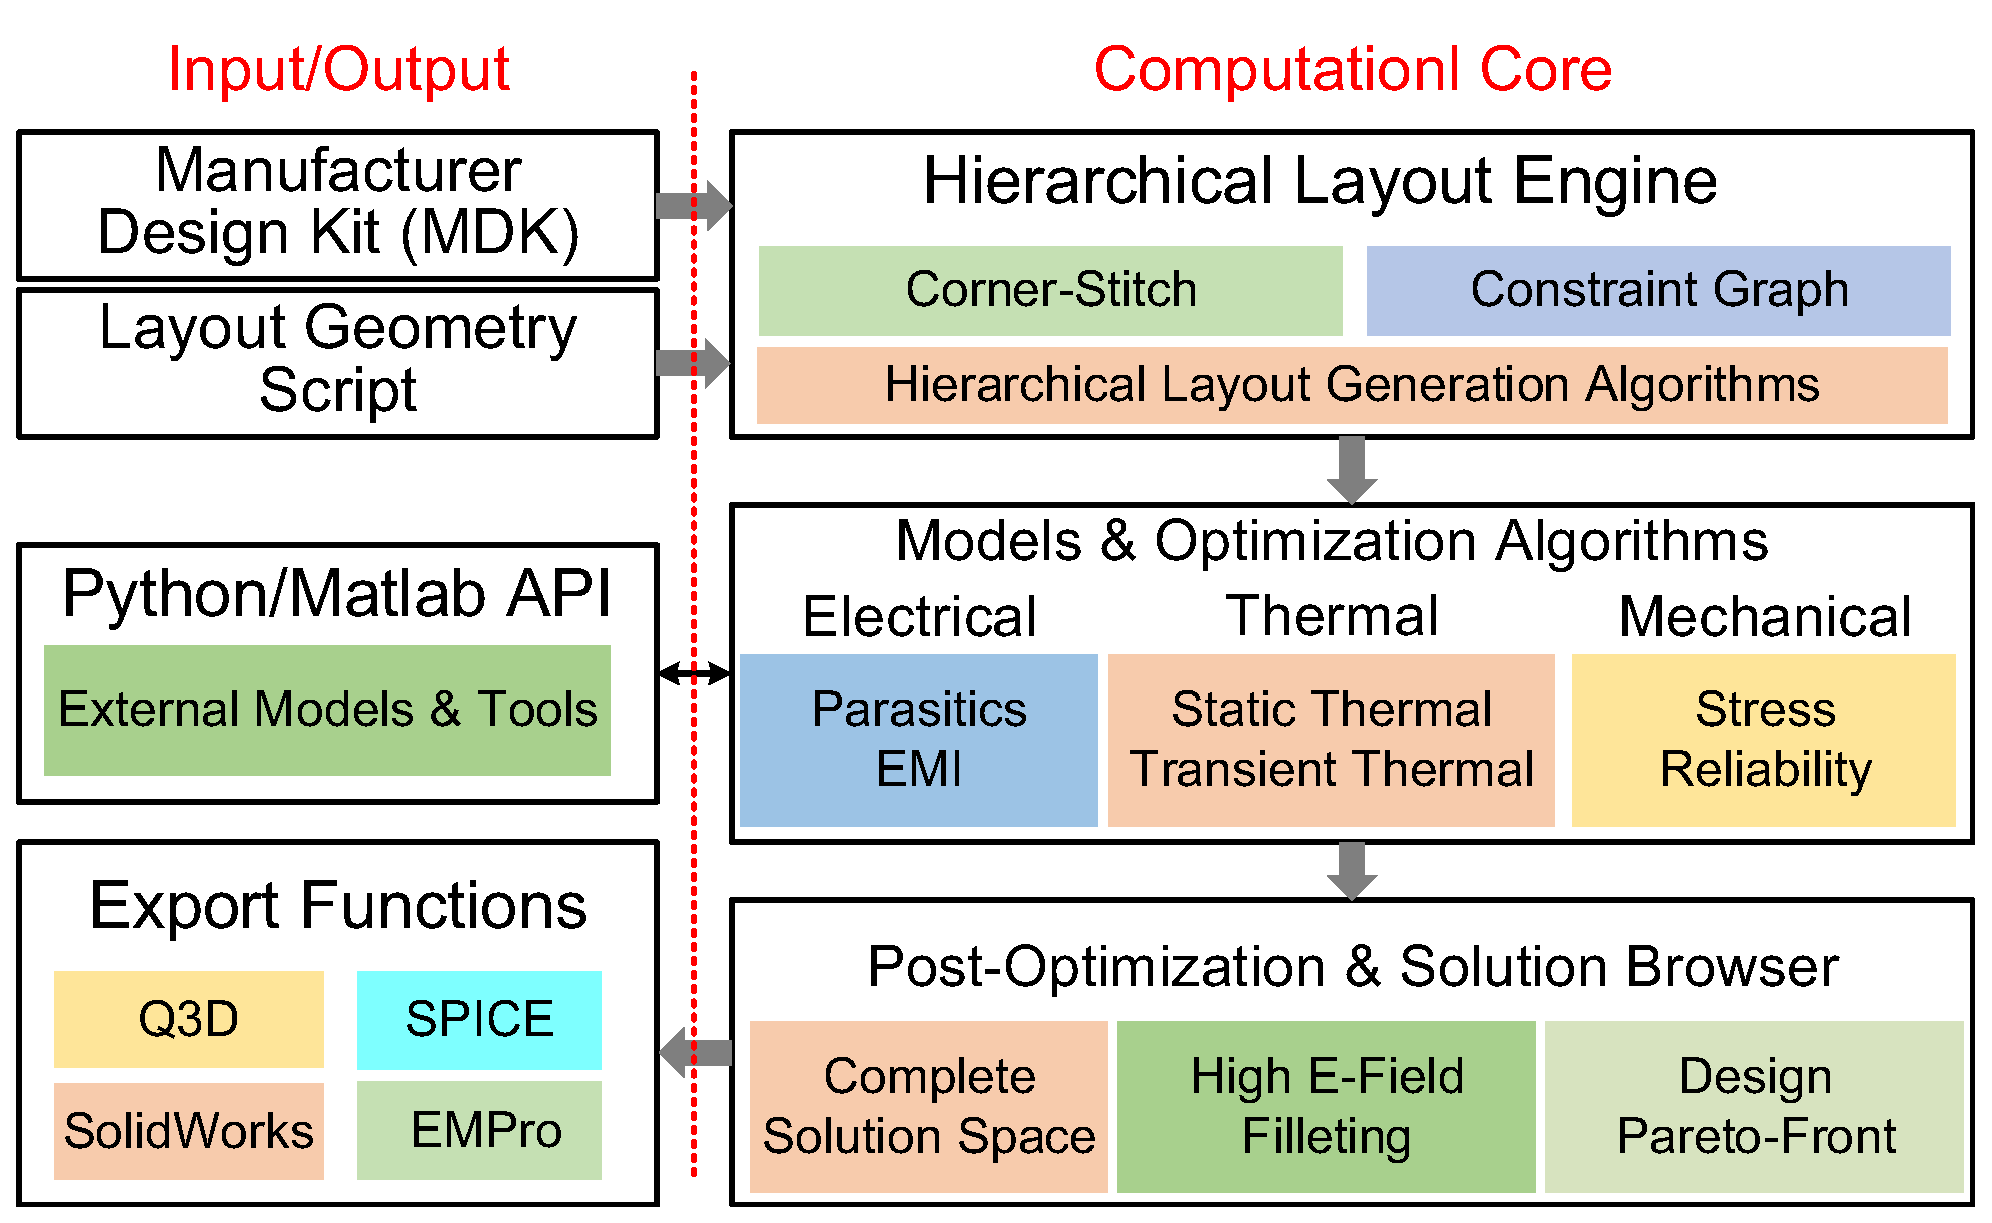
\includegraphics[width=\linewidth]{figs/v_1.9_figs/PS_overview.eps}
\caption{ PowerSynth architecture (v1.9)}
\label{fig:architecture}
\end{figure}

\subsubsection{Manufacturer Design Kit (MDK)}
In the Integrated Circuit (IC) design industry, the Process Design Kit (PDK) is one of the most important intellectual properties (IPs) from foundries to enable the design process. Similarly, for power module fabrication, a certain rule set has to be followed from the beginning of the layout design. This ruleset includes materials, devices, leads, bonding wires information, and design constraints with a technology layer stack. To ensure fabrication-ready layouts, a Manufacturer Design Kit (MDK) has been integrated with PowerSynth that contains an interactive material library, design constraints interface, and technology library. Since this version does not have a GUI to interact, the necessary information (materials, design constraints, layer stack) from the MDK are fed through CSV files. In stead of the technology library GUI, in this version, the components (devices, leads, bonding wires) information are taken through text files. Once the GUI is re-integrated with the upcoming version (v2.0), all those libraries will be interfaced with graphics. 


\subsubsection{ Hierarchical Constraint-Aware Layout Engine}
\label{sec-1-3-2}
The methodology of generating a layout solution is the backbone of the tool. In the latest version, the matrix-based methodology has been replaced by a more generic, efficient, and scalable one using the hierarchical corner stitch data structure with constraint graph evaluation techniques. This layout engine takes design constraints from the MDK together with an initial geometry script from the user as input to process the layout. With this methodology, an arbitrary number of components can be handled by applying generic and time-efficient algorithms. The significant improvements with the hierarchical constraint-aware layout engine are: 
\begin{itemize}
    \item An interactive constraint input feature which is helpful for user to specify or modify design constraint values to have different layout structures.
    \item Three types of layout generation capability: minimum-sized layout, variable floorplan sized, and fixed floorplan sized.
    \item As the engine takes into account of all design constraints in the layout generation phase, it always generates 100\% manufacture-able solutions.
    \item The updated layout engine can incorporate different types of optimization algorithms (i.e., genetic algorithm, gradient-based approach, stochastic approach, randomization)
    \item This layout engine treats each component as rectangle, so geometrical complexity is not a problem.
    \item This engine can process broader range of layouts even considering heterogeneous components (e.g. gate drivers, EMI filters, sensors, etc.).
    \item As the updated layout engine is constraint-aware, different types of constraints can be declared : design constraints, reliability constraints, user-defined constraints. Generated solutions always satisfy all the given constraints.

\end{itemize}
\textbf{Methodology}\\
From the user-defined initial input script, using corner stitch data structure (used in Magic VLSI tool), a collection of rectangular tiles are stored in a hierarchical tree structure. Based on design constraints, constraint graphs (popular in VLSI floorplan compaction) are created for each corner-stitched plane. Two types of constraint graphs are consdiered: horizontal constraint graph (HCG) and vertical constraint graph (VCG) for maintaining horizontal and vertical relationship among components. These constraints are evaluated using the longest path algorithm and the results are propagated through the tree. Bottom-up constraint propagation and top-down location propagation algorithms are implemented to generate solution. Detail algorithms can be found in \href{./Publications/I.Al.Razi-ECCE_19.pdf}{[13]}. Some concepts associated with layout generation are described as follows:

\begin{itemize}
\item \textbf{Constraints}:
Two types of constraints are considered: (a) design constraints, (b) reliability constraints.

\textbf{(a) Design Constraints:} These are standard design rules from the manufacturer. Three types of design constraints are considered.
\begin{enumerate}
    \item \textbf{Dimension Constraints}: Here, minimum width along x-axis (Min Width), minimum width along y-axis (Min Height) and minimum enclosure (Min Enclosure) are specified for each type of component. 
    \item \textbf{Spacing Constraints}: In this table, minimum spacing values between every pair of components are declared. 
    \item \textbf{Enclosure Constraints}: When a component is placed on top of another component, there may be some minimum enclosure value. So, this table has all possible minimum enclosure values.
\end{enumerate}
\textbf{(b) Reliability Constraints:} These constraints are user-defined based on the high-voltage-current applications. To minimize partial discharge phenomena, and increase the reliability of the power module, user can define voltage-dependent minimum spacing and current-dependent minimum width constraints.

\item \textbf{Operating Modes:}
Based on the evaluation of the constraint graphs, there are three modes of operation (shown in Table ~\ref{T.operating modes}).

\begin{table}[H]
\caption{Summary of operating modes}
\label{T.operating modes}
   \begin{tabular}{|c|c|c|}
\hline
\textbf{Mode} & \textbf{Purpose} & \textbf{Evaluation Methodology} \\ \hline
0 & Minimum sized layout & Minimum constraint values \\ \hline
1 & Variable floorplan layouts & \begin{tabular}[c]{@{}c@{}}All Weights are randomized with minimum constraints. \\ No maximum constraints\end{tabular} \\ \hline
2 & Fixed floorplan layouts & \begin{tabular}[c]{@{}c@{}}All Weights are randomized with minimum constraints. \\ Some have maximum constraints\end{tabular} \\ \hline
\end{tabular}

\end{table}
\begin{itemize}
    \item \textbf{Minimum Size Layout}: This layout is generated using all minimum constraint values. So, this layout reflects maximum possible power density for a layout. As this is the minimum sized solution, it is electrically optimized but thermal performance is so poor.
    \item \textbf{Variable Size Layout}: If this mode is selected, all constraint values are randomized and new layout solution is generated. User can generate arbitrary number of valid layout solutions with different floorplan size.
    \item \textbf{Fixed Size Layout}:  All edge weights are randomized within given area to generate arbitrary number of solutions. As floorplan size is always fixed there is less variation in this mode than the previous one.

\end{itemize}
\end{itemize}

\subsubsection{Performance Evaluation Models}
The electrical model has been updated to consider both self and mutual inductance, resistance, and capacitance. This is a PEEC-based model, which uses adaptive meshing and calculates parasitics more accurately than the previous response surface model. This model is described in \href{./Publications/Q.Le_IWIPP_19.pdf}{[12]}. The latest PowerSynth architecture is based on a modular approach so that the optimizer is flexible in accepting various models through application programming interfaces (APIs) while evaluating performance metrics. For example, the Army Research Lab (ARL) has developed a 3D thermal and stress evaluation tool called ParaPower. To incorporate their thermal and stress model, a PowerSynth-ParaPower API has been developed to allow PowerSynth to use ParaPower for thermal and stress evaluations. However, in this version, this model has not been incorporated as the PowerSynth fast thermal model (described in \href{./Publications/PowerSynth-A_Module_Layout_Generation_Tool.pdf}{[11]}) is accurate and faster for any 2D/2.5D module. The ParaPower stress and thermal model, and another SPICE-based transient thermal model will be incorporated in the next release.

\subsubsection{Optimization Algorithm}
In this version, the built-in solution generator algorithm "Non-guided randomization"(\href{./Publications/WIPDA_2018.pdf}{[10]}) has been provided as an optimization algorithm. Though this algorithm does not account for any specific objective, this can generate a larger solution space than the genetic algorithm, which can eventually find a better solution. The genetic algorithm implementation is on-going and will be incorporated in the upcoming release.


\subsubsection{Post-Optimization and Solution Export}
In this version, along with the Pareto-front solutions, an entire solution space is also reported after optimization. Moreover, for each solution, the layout geometry is also exposed in a CSV file containing each component's coordinates, width, and length. This information helps a designer to regenerate the geometry script for the solution layout. Though the automatic export to commercial FEA tools like ANSYS Q3D, and SolidWorks feature is disabled in this command line version,
it will be back with the next release GUI version.

\section{Using PowerSynth v1.9}
\label{sec-2}

\subsection{Installing and Running PowerSynth v1.9}
\label{sec-2-1}
To install PowerSynth v1.9, run the PowerSynth install wizard. It will take some time to install. Upon installation, the user can run PowerSynth v1.9 executable.\\
\textbf{Note:} It is STRONGLY RECOMMENDED that you install PowerSynth in the C drive (the default installation directory) and NOT in Program Files. Installing PowerSynth in Program Files can result in various issues relating to administrator permissions.\\
To run the commandline version, the steps are as follows:\\
1. Start a command prompt as administrator.\\
2. Go to the directory of \textbf{"PowerSynth.exe"}.\\
3. Run PowerSynth by entering the command: PowerSynth.exe.\\
4. The command prompt will ask for the location of the \textbf{"Settings.info"} file. This file is already provided with the package.\\
5. Upon entering the location of the \textbf{"Settings.info"} file, hit enter.\\
6. Now, it will ask for the \textbf{"Macro script"} file location.\\
7. Sample \textbf{"Macro script"} is provided in the \textbf{"Sample\_Projects"} folder inside the package. You can use any of the test case macro script file location to test it or you can create your own test case. Details of preparing a \textbf{"Macro script"} are described in Section~\ref{sec-2-2}.\\
8. Upon entering the \textbf{"Macro script"} file location, PowerSynth will execute necessary steps according to the option specified in the \textbf{"Macro script"}.

So, to run PowerSynth v1.9, user needs to files: (a) \textbf{Settings file}, and (b) \textbf{Macro script}. Since the \textbf{Settings file} is provided with the package, the user needs to create a \textbf{Macro script} only to run a layout optimization. So, in the following subsections, the \textbf{Macro script} prepartion details are described.

\subsection{Requirements}
\label{sec-2-2}

\subsubsection{Technology Library Content}
\label{sec-2-2-1}
To design a standard 2D/2.5D power module (shown in Figure~\ref{power_module}), the key elements are as follows:\\
1. Baseplate\\
2. Substrate (Direct Bonded Copper (DBC): Back-side metal, Ceramic, Top-side metal)\\
3. Components (Devices: MOSFETs, Diodes, IGBTs, Capacitors, etc.)\\
4. Connectors (Leads: power and signal)\\
5. Bonding wires.\\

\begin{figure}[t]
\centering
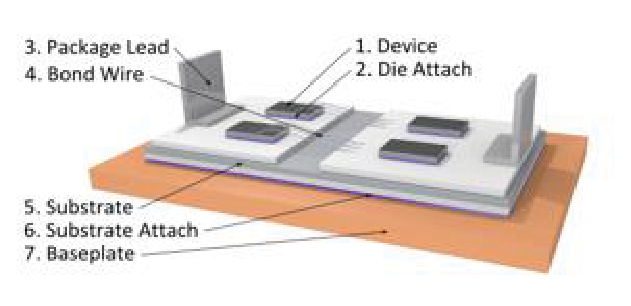
\includegraphics[width=4 in, height=2 in]{figs/v_1.9_figs/module_struct.eps}
\caption{Standard 2D power module}
\label{power_module}
\end{figure}

Since the technology library is not integrated with this version, these elements information are taken through files. The files associated with these elements are as follows:\\
1. Layer stack (.csv file)\\
2. Parts (.part file)\\
3. Wires (.wire file)\\
4. Constraints (.csv file)\\
Each file content is described below:
\begin{enumerate}

\item \textbf{Layer stack:} This file provides the dimensions, material information about baseplate, and substrate. These information are taken input as a CSV file. A sample layer stack is shown in Table~\ref{layer_stack_example}. The file has eight columns:\\
    1. ID: An integer to uniquely identify each layer.\\
    2. Name: Each layer needs to have a name (i.e., B1 for Baseplate layer 1, M1 for substrate backside metal 1, D1 for dielectric layer 1 of the substrate, I1 for interconnect layer 1 of the substrate, and C1 for component layer 1). Since this version supports multi-layer stacked DBC, all layers except the component layer can be multiple.\\
    3. Width: Defines width of each layer in mm.\\
    4. Length: Defines length of each layer in mm.\\
    5. Thickness: Defines thickness of each layer in mm.\\
    6. Material: Name of the corresponding layer material (needs to be same as in material library (i.e., MATERIAL\_LIB\_PATH in the settings.info file)).\\
    7. Type: Two types are allowed: p for passive and a for active. Only component layer is an active layer and rest of the layers are passive.\\
    8. Electrical: This field is for electrical performance evaluation. Here, F for floating, G for ground, D for dielectric, S for signal, and C for component.



    \begin{table}[H]
      \centering
      \caption{Content in a layer stack file}
    \begin{tabular}{|c|c|c|c|c|c|c|c|}
    \hline
    ID    & Name  & Width & Length & Thickness & Material & Type  & Electrical \bigstrut\\
    \hline
    1     & B1    & 50    & 60    & 1     & copper & p     & F \bigstrut\\
    \hline
    2     & M1    & 42    & 52    & 0.2   & copper & p     & G \bigstrut\\
    \hline
    3     & D1    & 40    & 50    & 0.64  & Al\_N & p     & D \bigstrut\\
    \hline
    4     & I1    & 40    & 50    & 0.2   & copper & p     & S \bigstrut\\
    \hline
    5     & C1    & 40    & 50    & 0.18  & None  & a     & C \bigstrut\\
    \hline
    \end{tabular}%
  \label{layer_stack_example}%
\end{table}%


Since, this version supports only layer-based geometry, the component layer (ID=5 in Table~\ref{layer_stack_example}) thickness and material information are optional.

\item \textbf{Parts:} The components (devices) and connectors (leads) are considered as parts in this version. The dimensions, material information of these elements are taken from corresponding .part file. These files are written in a text editor and saved as .part extension. A sample MOSFET.part and power\_lead.part file content are shown in Figure~\ref{component_file} (a), (b), respectively. 
    \begin{figure}[H]
    \centering
    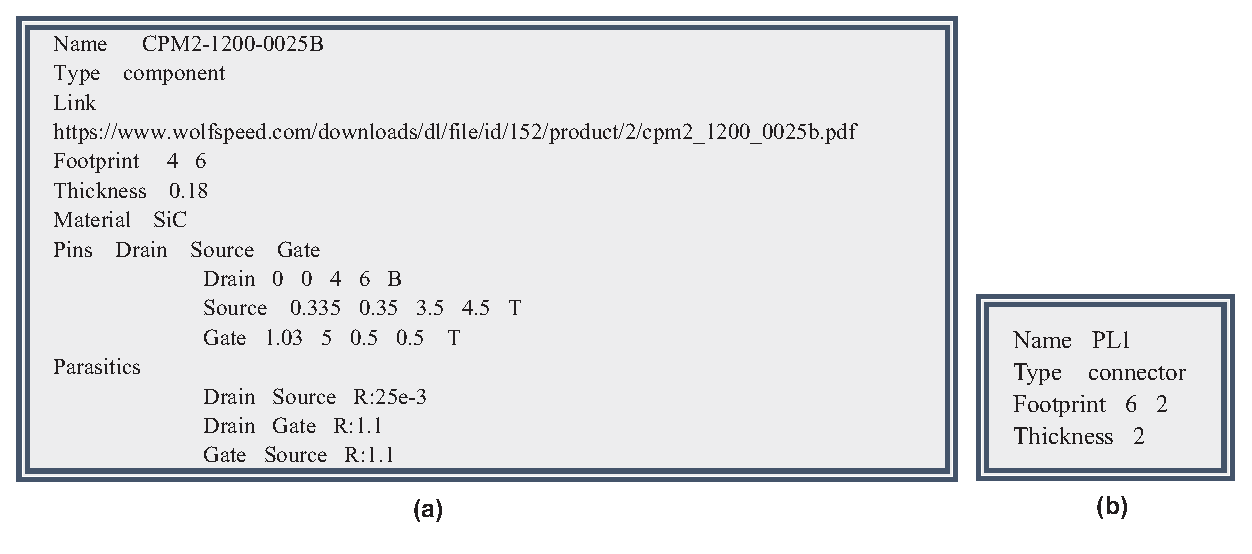
\includegraphics[width=\linewidth ]{figs/v_1.9_figs/comp_con.eps}
    \caption{Content in (a) MOSFET.part, (b) power\_lead.part file }
    \label{component_file}
    \end{figure}
    
In  Figure~\ref{component_file} (a), each row has a key name e.g. “Name” and a value separated by a space e.g.: “CPM2-1200-0025B”. The definition for each key is as follows:\\
    Name: Name of the Part\\
    Type: There are 2 options: component (device like MOS, diode, capacitor, etc.) or connector (terminals like power lead, signal lead, etc.)\\
    Link: A link to the part datasheet\\
    Footprint: Width <space> Length (Provide the footprint of the component in mm)\\
    Thickness: Thickness of the component (in mm)\\
    Material: Name of the Material (e.g., SiC) [should match with material library from MDK (materials.csv file in MATERIAL\_LIB\_PATH of "settings.info" file.)]\\
    Pins [list of preferred pin names separated by space]: Provide a list of pin names\\
    Pin\_name: For each pin provide a pin pad rectangle (bottom-left coordinate x <space> y <space> width <space> height) reference to the component bottom left corner. At the end of the pin rectangle add a keyword B or T to distinguish between Bottom and Top side pins.\\
    Parasitics: Used to provide component internal parasitic information.\\
	Pin\_name1 <space> Pin\_name2 <space> R: R\_val <space> L:L\_val <space> C:C\_val\\
	Provide a list of RLC value between every 2 pins (with internal parasitics)
	
	For different devices, the keys need to be same, but the values will be changed depending on the device type. 
	In  Figure~\ref{component_file} (b), each row has a key, value pair separated by a space.The definitions for each key are similar to those in  Figure~\ref{component_file} (a).
	
	In this version, the footprint dimensions declared in the .part files need to be always integer. However, the user can change the footprint dimensions into the floating point numbers in the constraint file (described in the "Constraint File" section). Also, all .part files need to be saved in the "Part\_Lib" folder. More sample .part files are provided in the "Sample\_Projects" folder inside "Part\_Lib".

\item \textbf{Wires:}  The wire standard, resistivity, and radius information are stored in a *.wire file. The file content are written in a text editor and saved as .wire extension. Content of a sample wire file is shown in Figure~\ref{wire_def}.
    \begin{figure}[H]
    \centering
    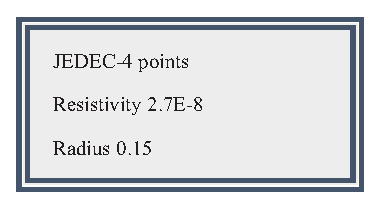
\includegraphics[width=2 in, height=1 in]{figs/v_1.9_figs/bw_info.eps}
    \caption{Content in a *.wire file}
    \label{wire_def}
    \end{figure}
    
In the *.wire file, the first line is the wire bonding standard. This will affect the parasitic extraction of the bond wire group. The second line is the resistivity of the material. This is used to compute the parasitic resistance of the wire (unit is \textohm m). The third line is used to provide the radius of the wire in mm. For bond wire with square cross section, the effective radius can be used. In the last two lines, there is a space in between key and value. All *.wire files need to be saved in "Wire\_Lib" folder. \\

\item \textbf{Constraints:}
The minimum constraint values are given as input through a CSV file. Generally, for each layout the constraint file is automatically populated with some default values. However, the user can always modify the values according to the manufacturer requirements. Since in this version, two types of constraints (i.e., standard design constraints, and reliability constraints) are considered, the default constraint table generates minimum standard design constraints and the user needs to set a flag (\textbf{`Reliability-awareness'}) to indicate that the reliability constraints are available (high voltage application). The description about the flag usage is in Section~\ref{sec-2-3}. The default constraint file content for the sample layout in Fig.~\ref{layout_script} is shown in Fig.~\ref{cons_values_new_0_rel_0}.

    \begin{figure}[H]
    \centering
    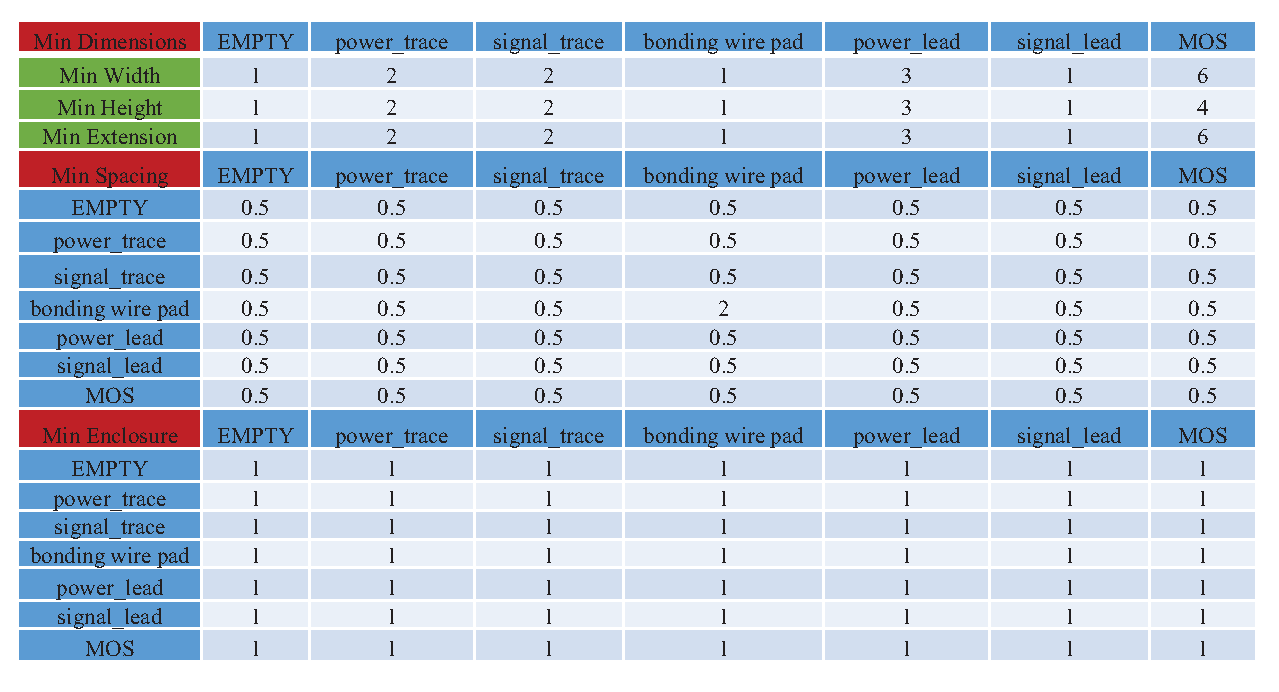
\includegraphics[width=\linewidth ]{figs/v_1.9_figs/cons_1.eps}
    \caption{Content in a constraint file with minimum design constraints only}
    \label{cons_values_new_0_rel_0}
    \end{figure}
In Figure~\ref{cons_values_new_0_rel_0}, the highlighted (red/green) fields are representing constraint names. The blue colored fields are representing the elements in the layout. All elements are directly related to the layout geometry description script (shown in Figure~\ref{layout_script}) except the \textbf{"EMPTY"} field. This type represents the etched area on top of a DBC, which means any area where there is no copper. Rest of the fields are for constraint values. In any power module, in this PowerSynth version, it is assumed that there will be at least three elements: power trace, signal trace, and bonding wire pad. Rest of the elements are dynamically changing depending on the initial layout. For example, in the Figure~\ref{cons_values_new_0_rel_0}, there are power lead, signal lead, and MOS because the corresponding layout description script from Figure~\ref{layout_script} has three components in the \textbf{`\# Definition} section. If any layout has more components or other components, the corresponding fields will appear in the constraint file.


If the \textbf{Reliability-awareness} flag is set, then along with the minimum design constraints shown in Figure~\ref{cons_values_new_0_rel_0}, additional content is populated in the same constraint file. The additional rows in the csv file for the sample layout in Figure~\ref{layout_script} is shown in Figure~\ref{cons_values_new_0_rel_2}. Here, first few lines are for voltage and current specifications with default value 0. The user needs to modify the values according to the specific requirements. In the voltage and current specification sections, there are four fields to describe the voltage and current loading for each island (connected group of traces) as all waveforms are considered in generic sinusoidal form: A+ B sin ($2\pi ft+\theta$). Here, A= DC magnitude (V/A), B= AC magnitude (V/A), f= Frequency, $\theta$ = Phase angle. So, while providing the values, the waveform needs to be fit in the equation and then the coefficient values need to be provided. If there are multiple traces in an island, one trace will be appeared in the constraint table as all traces on the same island are connected. For example, in the constraint table shown in Figure~\ref{cons_values_new_0_rel_2}, only \textbf{T1.4} has appeared as \textbf{T1.4, T2.4, and T3.4} are on same island in Figure~\ref{layout_script}.\\
Once the waveforms are defined, the voltage-dependent minimum spacing and current-dependent minimum width values need to declared in the last two sections (highlighted in red color). For voltage difference vs minimum spacing, user can add rows depending on the expected voltage difference levels in the layout. The voltage difference calculation method can be found in \href{./Publications/Y.Peng_NOLTA_20.pdf}{[15]}. For example, if the user is expecting 3 voltage differences like 0V, 1000V, 2000V, three rows need to be added in this section with the corresponding minimum spacing values. Similarly, for the current rating vs minimum width constraints, user needs to add rows depending on the requirements. The voltage differences and current ratings in the constraint table need to increase with a constant value. If the calculated voltage difference between two traces is in between two values provided in the constraint table, it will choose the upper bound for safety. For example,  if the user has 0 V, 1000 V, 2000 V voltage differences, and the calculated voltage difference is 1500 V, the constraint value that will be applied is for the 2000 V difference case.

    \begin{figure}[t]
    \centering
    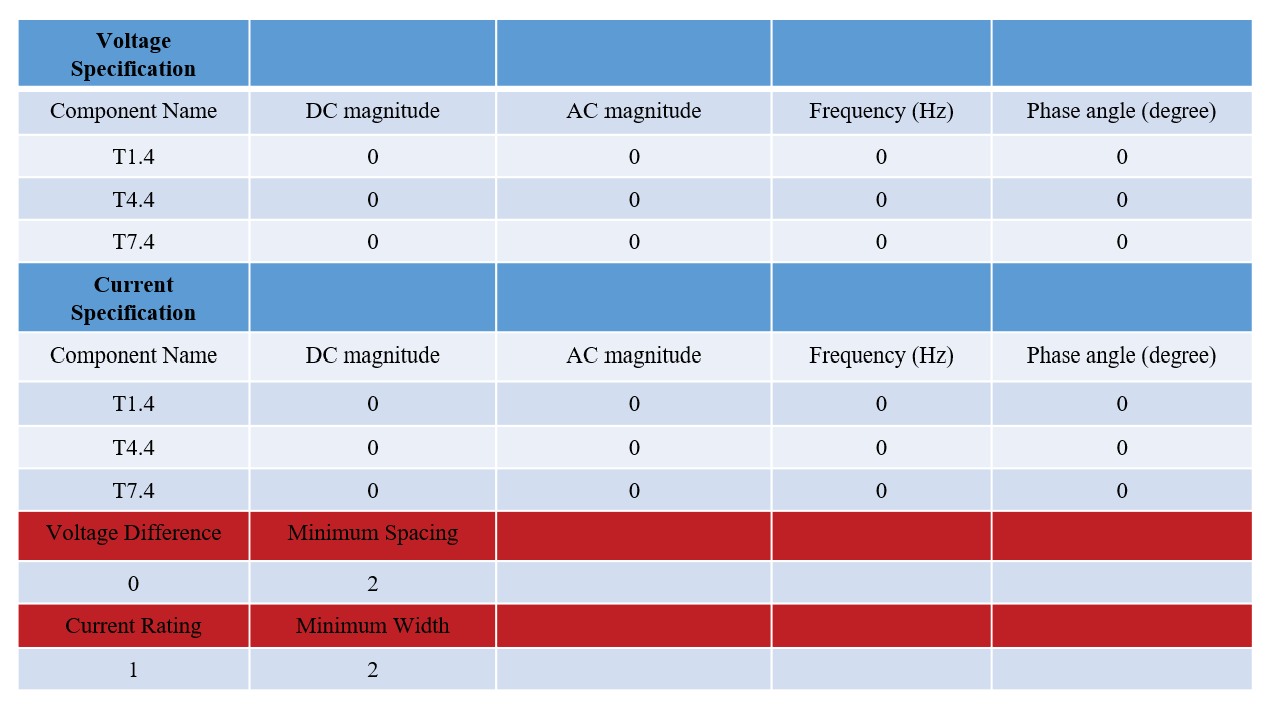
\includegraphics[width=\linewidth ]{figs/v_1.9_figs/cons_2.eps}
    \caption{Content in a constraint file associated with the reliability constraints}
    \label{cons_values_new_0_rel_2}
    \end{figure}

 The user can open the constraint file and edit the values and save it in the same location. No renaming is required. While assigning the constraint values, care needs to be taken to make sure the constraints are valid.  

\end{enumerate}

\subsubsection{Initial Layout Description}
\label{sec-2-2-2}
Once the technology library related files are ready, the initial layout needs to be described through the text (.txt) files. Two files are required to describe an initial layout of a power module:\\
1. Layout geometry description script\\
2. Bonding wires connection description file.\\
Each of the file content is described below in detail:
\begin{enumerate}

    \item \textbf{Layout geometry description script:} This script is a text (.txt) file to input the initial layout geometry of the layout. This script contains the initial placement and routing of the components, and connectors. A sample script file content is shown in Figure~\ref{layout_script}.
    \begin{figure}[t]
    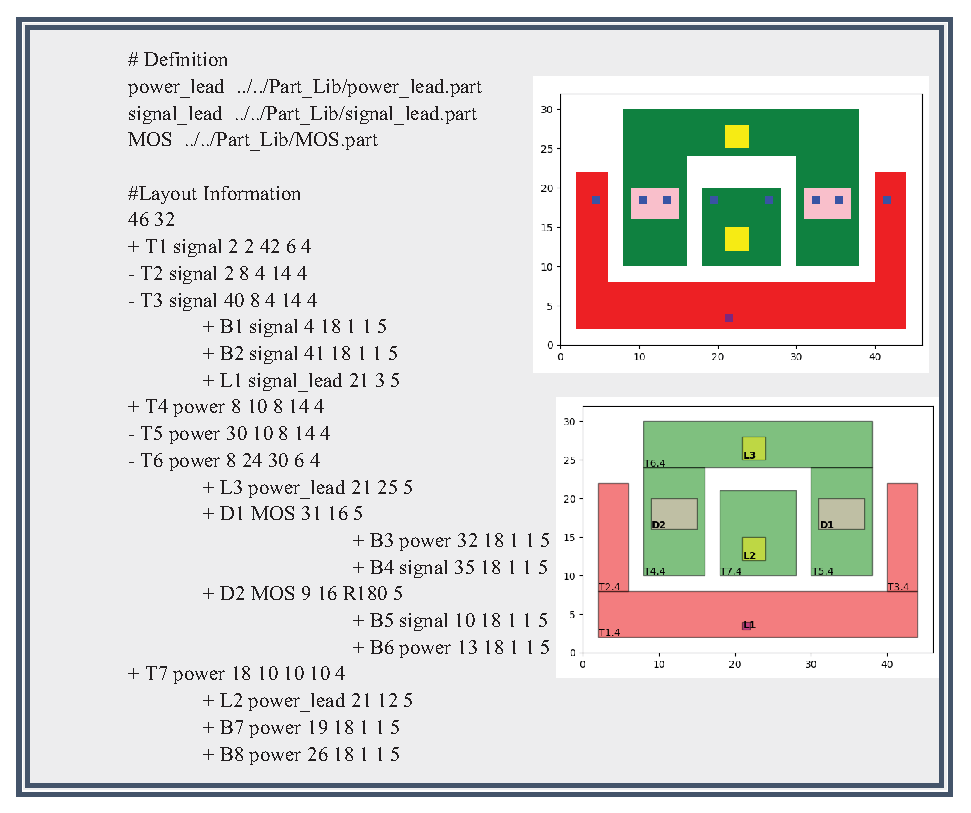
\includegraphics[width=\linewidth]{figs/v_1.9_figs/init_layout.eps}
    \caption{Content in a layout geometry description script}
    \label{layout_script}
    \end{figure}
    The file has two sections:\\
    \textbf{(a) Definition}\\
    In this part, the necessary parts (.part) file locations are provided. Anything below the tag “\#Definition” and up to the tag “\#Layout Information" in the script are considered in this section. For any new test case, the tags should not be changed. Also, a blank line is required in between two sections (as shown in Figure~\ref{layout_script}).\\
    The user can use any keywords to represent a component or connector which is defined by the *.part file. These keywords need to be reused in the “\#Layout Information" section. In the “\#Definition” section, in each line, there are two segments:\\ <segment1> <space> <segment2>.\\
    <segment1> is the keyword of the component or connector (MOS, Diode, IGBT, power\_lead, signal\_lead, etc.)\\
    <segment2> is the relative location of the component.part file.\\\\
    
	\textbf{(b) Layout Information}\\
	This section describes the layout geometry and component hierarchy information for the layout engine. Anything below the tag “\#Layout Information” are used to describe the layout geometry. The geometry should be described hierarchically and the hierarchical order is bottom-to-top. For example, in the sample script shown in Figure~\ref{layout_script}, T4, T5, T6 are connected traces and together create an island. This island should be declared first and then the devices or leads on top of it need to be declared. Each island can be composed of single or multiple traces. All connected traces in the same island needs to be declared at same hierarchy level. The declaration should start with a ‘+’ character and other connected components need to start with a ‘-‘ character. All components in each connected group should be of the same type (i.e., power traces or signal traces).

    Each hierarchy level is separated by a ‘tab’ in the script and we currently support up to 3 levels of hierarchy (2 tabs) in this version (Trace->Device->Pin). Also, in the input script, the coordinates should be given as integer values. However, in the constraint table, the fractional constraint value is allowed up to 3rd decimal point.

    All of the width and height information for devices or leads are directly read from the corresponding “.part file” mentioned in the \textbf{Definition} section. So, these components do not have width or height information specified in the layout geometry description script, whereas others (e.g., traces and bond wire pads) have width and height fields.

    To have a bond wire, the source pad and destination pad of the bond wire needs to be aligned according to the wire orientation. For example, in the sample script (shown in Figure~\ref{layout_script}), the gate signal is connected from B4 to B2 (\textbf{Bonding wires connection description file} section). B4 is on top of the gate pad of D2. So, B4 and B2 should have the same y coordinate as this represents a horizontal bond wire connection.
    The bond wire pad is always a square with size of 1 mm in the input script, even though it is considered as a point connection in the algorithms.
    
    Description of each line in the \textbf{'\#Layout Information'} section:\\
    Line1: size of initial layout (width (along X-axis), height (along Y-axis))\\
    Line2-to-end: each line has several fields:\\
    For all routing paths (Traces, Bond wire pads) have 8 fields:\\
    1.	‘+/-’ : Connectivity definition character\\
    2.	‘ID’ : layout component id (T1: Trace 1, T2: Trace 2, B1: Bond wire pad 1,etc.)\\
    3.	‘type of component’: for traces, bond wire pads-> power or signal\\
    4.	x coordinate: bottom left corner’s x coordinate\\
    5.	y coordinate: bottom left corner’s y coordinate\\
    6.	width: width of the rectangle (along x axis)\\
    7.	height: height of the rectangle (along y axis)\\
    8.	layer\_id: id of the layer(value is taken from the layer stack)\\
    For all parts (Devices, Leads) have 6-7 fields:\\
    1.	‘+/-’ : Connectivity definition character\\
    2.	‘ID’ : layout component id (D1: Device 1, L1: Lead 1,etc.)\\
    3.	‘type of component’:\\
    for devices-> name (should match with definition part)
    (MOS,Diode, IGBT, etc.)\\
    for leads-> name of lead (power\_lead or signal\_lead or neutral\_lead)\\
    4.  x coordinate: bottom left corner’s x coordinate\\
    5.	y coordinate: bottom left corner’s y coordinate\\
    6.	Rotate angle: R90(90\textdegree rotation), R180(180\textdegree rotation), R270(270\textdegree rotation)\\
    7.	Layer\_id: id of the layer(component layer id in the layer stack)\\
Please note that in this release, while creating a new layout geometry description script, no extra space/tab/new line is allowed after each line and at the end of the script. Also, the coordinates of the elements on the same island (connected group) are correlated to each other. To get the best results, this coordinate correlation needs to be minimized in the initial layout description script. For better results, the bond wire coordinates should not be correlated with any other coordinates. To test if the updated constraints and initial layout description script are valid, please generate a minimum-sized solution. If there is an error in layout generation, the constraint values may not be feasible. Also, if the minimum-sized solution is not a feasible one, there is probably a correlation issue. Try to break correlations in the input script and run again. This can be a trial and error process where the user needs to play with the input script until a feasible minimum-sized solution is found.
    
    
    \item\textbf{Bonding wires connection description file:}
    This is a text (.txt) file that defines all bonding wire connections. An example of the file content is shown in Figure~\ref{wire_setup_table}.
    This file has two parts:\\
    \textbf{(a) Definition}\\
    This section starts with a tag \textbf{`\# Definition'}. In this section, different types of wire file (*.wire) locations are described. In each line, there are two segments: \\
    <segment1> <space> <segment2>\\
    <segment1> is the wire name (used to map in the \textbf{Table\_info} section).\\
    <segment2> is the relative location of the wire file (.wire). This file content is described in \textbf{Wires} in Section~\ref{sec-2-2-1}.
    
    \textbf{(b) Table\_info}\\
    From the initial layout, the user needs to connect each wire between its respective landing pins. Some of the pin names are mentioned inside the component (*.part) file. For example, a MOS with keyword D1 will have 3 pins: D1\_Drain, D1\_Source, and D1\_Gate. Also, other pins are shown in the layout file (Figure~\ref{layout_script}), such as B1, B2,..., etc. are used as bonding wire landing pads. 
    
    
    \begin{figure}[hbt]
    \centering
    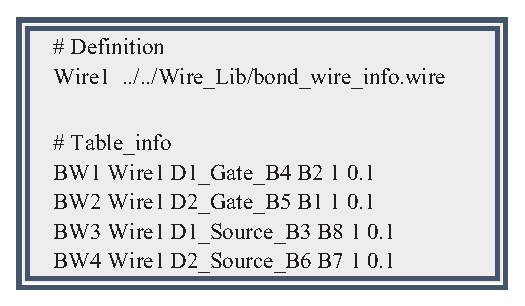
\includegraphics[width=3.5 in]{figs/v_1.9_figs/bw_table.eps}
    \caption{Content in a bonding wire connection description file}
    \label{wire_setup_table}
    \end{figure}
    
    Similar to the \textbf{Definition} for the components in the layout script, the user can use any keywords for different types of wires. For each row under the \textbf{\# Table\_info} tag, the user can define a bonding wire group (a set of parallel wires), begin with a name for the group, wire definition, start pin name, end pin name, number of wires, and spacing (in mm) among multiple wires in the group separated by a space. For the example shown in Figure~\ref{wire_setup_table}, the first line in the \textbf{\# Table\_info} section defines a bonding wire with name: `BW1', type: `Wire1', start pin: `D1\_Gate\_B4', end pin: `B2', number of wires: `1', and spacing: `0.1'. Since B4 and B2 are connected, in the layout script (shown in Figure~\ref{layout_script}) they have same Y-coordinate as this wire is a horizontal wire. Also, B4 represents the gate pin of the device D1, so the start pin name is `D1\_Gate\_B4'.
    
\end{enumerate}

\subsection{Macro Script Content}
\label{sec-2-3}
In a macro script there are two major sections:
\begin{enumerate}
    \item Input Scripts
    \item Layout Generation and Optimization Setup
\end{enumerate}
Description about each section is as follows:
\subsubsection{Input Scripts}
\label{2-3-1}
In this section, eight files/directories locations are provided. Detailed description for each of them are provided below:
\begin{enumerate}
    \item \textbf{Layout\_script:} In this field, the relative location of the \textbf{Layout geometry description script} (described in Section~\ref{sec-2-2-2}) needs to be provided.
    \item\textbf{Bondwire\_setup:} Here, the relative location of the \textbf{Bonding wires connection description file} (described in Section~\ref{sec-2-2-2}) needs to be provided.
    \item \textbf{Layer\_stack:} Relative location of the \textbf{Layer stack} file (described in Section~\ref{sec-2-2-1}) is provided here.

    \item \textbf{Parasitic\_model:}
    In this version, only PEEC-model is embedded for electrical parasitics extraction. Some sample files are given for the test cases in 'Sample\_Projects' folder with the package. Please, note that for different layouts, if you experience very large or negative values during resistance and inductance extraction, a new model is needed. Please contact the developers if you are getting weird parasitic values for your case as the interface of creating a new model file is not provided in this version.
    
    \item \textbf{Fig\_dir:}
    Needs a relative path of a directory to save the figures.
    \item \textbf{Solution\_dir:}
    Needs a relative path of a directory to save the solution database file. This database file contains layout information which is used to plot the figures. In this folder, all performance values of the solutions and corresponding Pareto-front solution set are reported as a .csv format. Besides, two folders will be created, where each layout solution components and corresponding coordinates, dimensions of all solutions and Pareto solutions are dumped in individual CSV file.
    
    \item \textbf{Constraint\_file:}
    The constraint file is a CSV file, where all constraint values are stored. Depending on the mode of the flag \textbf{`New'} in the macro file (described in Section~\ref{sec-2-3-2}), a constraint file will be created or loaded to generate the layout solutions. In this field, the user needs to provide the relative location of an empty CSV file (for the first time for each layout) and make sure the \textbf{'New'} flag is set to 1. This flag value allows user to modify the default constraint values populated by PowerSynth. Once the values are modified, the \textbf{'New'} flag needs to be set to 0, which reloads the constraint values in the specified file and does not require to edit the values again. The file content is described in Section~\ref{sec-2-2-1}.
    
    \item \textbf{Trace\_Ori:}
    This field is the 'Trace Orientation' description file. A text (.txt) file relative location with trace orientations needs to be provided. This file is required for the electrical model to evaluate electrical performance. Two orientations are possible for each trace: Horizontal and Vertical. This represents the preferred current flow direction for the trace.\\
    The format for the file content is as follows:\\
    H: Horizontal trace\_1 name.layer\_id, Horizontal trace\_2 name.layer\_id, ……, etc.\\
    V: Vertical trace\_1 name.layer\_id, Vertical trace\_2 name.layer\_id, ……, etc.\\
    Here, layer\_id is the last field in that trace geometry definition line in \textbf{Layout\_script}.\\
    For example, the layout shown in Fig.~\ref{layout_script}, the Trace\_Ori.txt file content is:\\
    H: T1.4,T6.4\\
    V: T2.4,T3.4,T4.4,T5.4,T7.4\\
    
\end{enumerate}
\subsubsection{Layout Generation and Optimization Setup}
\label{sec-2-3-2}
\textbf{Layout Generation}\\
In this section, PowerSynth layout solution generation and performance evaluation setup are defined. PowerSynth v1.9 can serve three purposes:\\
1. Layout solution generation only.\\
2. Initial layout performance evaluation.\\
3. Layout optimization: solution generation and performance evaluation.\\
Each field for this section is described below:
\begin{enumerate}
    \item \textbf{Reliability-awareness:}
    If high-voltage and current dependent constraints (reliability constraints) are available and the user wants to apply those, this flag should be set to 2. Setting up this flag as 0 indicates no reliability constraints are applied. If this flag is set to 1, worst-case conditions (theoretical, not always practical) are considered. To have reasonable, practical, and reliability-aware layout generation, this flag needs to be set to 2. If reliability-awareness is set to 1, or 2, in the constraint table, voltage and current specifications are populated for modification. Details are described in Section~\ref{sec-2-2-1}. 
    
    \item \textbf{New:}
    If \textbf{`New'} flag is set to 1, user will be asked to edit the constraint table in the given constraint file location while running the test case. Once the edition is done, user needs to enter "1" in the terminal to continue. For each new test case, this flag has to be set to 1 for the first run. Then, for other iteartions, the flag needs to be set to 0, otherwise the modified constraint values will be overwritten by the default values. If the flag is set to 0, the constraint values already saved in the given constraint file are used to generate solutions.
	
	 \item \textbf{Plot\_Solution:}
	 If this flag is set to 1, all solution layout images will be saved in the \textbf{Fig\_dir}. This is only recommended for small solution spaces (<100 layouts). For large solution spaces, plotting each figure will cause memory issue in matplotlib. So, this flag should be set to 0.
	 
	 \item \textbf{Flexible\_Wire:}
	 If this flag is set to 0, the bonding wires are rigid (i.e., needs to be strictly horizontal or vertical). In the \textbf{Layout\_script}, any connected pair of bond wire pads need to be declared carefully to maintain their orientation alignment. For example, if the bond wire is horizontal, the start and end pins of the wire need to be horizontally aligned (same y coordinates). Also, in the \textbf{Bondwire\_setup} file, the connection is allowed only between bond wire pads.
     If the flag is set to 1, flexible bond wires are considered. A flexible bond wire is one that can be connected between any two points in the layout. There is no restriction on the orientation (i.e., horizontal, or vertical). In this case, the \textbf{Layout\_script} and \textbf{Bondwire\_setup} file need to compatible with the flexible wire implementation. For flexible bond wires, in the layout script, no bond wire pad is allowed on top of the device. So, in the bond wire connection table, the wires having source or destination as a device, needs to be only pad (as declared in part definition).
     However, the flexible wire would overestimate the bonding wire length and so this feature is not available for the users. So, default value is set to 0 and it is recommended not to change the value. If you want to use this feature, please contact developers.
     
     \item \textbf{Option:}
     To choose from the three options mentioned earlier: 1. Layout solution generation only, 2. Initial layout evaluation, 3. Layout optimization/evaluation, this flag is provided. Based on your choice provide 0, 1, 2 respectively for the options given above. For example: to run layout optimization, you will provide 2 in the option field. Initial layout does not guarantee design rule check (DRC) clean solution as it is described by the user. Other options generate solutions by considering design conatraints and hence they are DRC-clean. 
     
     \item \textbf{Layout\_Mode:}
     This field is related to layout generation. In this version, three modes of layout generation are allowed: 1. Mode-0: minimum-sized solution, 2. Mode-1: variable-sized solutions, 3. Mode-2: fixed-sized solutions. Details are described in Section~\ref{sec-1-3-2}. This option is effective if the user 
     has chosen 0 or 2 as \textbf{Option} field value. For Mode-0, a single solution is generated. For other modes user can choose number of solutions. Since in Mode-0, user can generate a single solution, if \textbf{`Option'} is set to 2, that single solution will be evaluated and this will not generate any Pareto-front as the solution space length is 1. It is recommended that for each new test case, user generates minimum-sized solution (Mode=0) to make sure that the initial layout and constraint values are correct. However, based on user requirement, \textbf{Layout\_Mode} value can be 0, 1, or 2. For example: if user chooses fixed size layouts to be generated, \textbf{Layout\_Mode} should be set to 2.
	 There are some other parameters required depending on the \textbf{Layout\_Mode}: Seed, Floor\_plan, Num\_of\_layouts.
	 
	 \item \textbf{Seed:}
	 Randomization seed. Effective for \textbf{Option}=0, and 2 and \textbf{Layout\_Mode}= 1, 2. Because for the rest of the mode/option there is a single solution.
	 
	 \item \textbf{Floor\_plan:}
	 Size of layout (Width, Height). This input is effective for \textbf{Option}=0, and 2 and \textbf{Layout\_Mode}= 2. Because the Mode-2 generates the fixed floorplan size solutions. Please make sure that the input floorplan size is larger or equal to the minimum floorplan size.
	 
	 \item \textbf{Num\_of\_layouts:}
	 Desired number of solutions. Need to give an integer. Required for \textbf{Option}=0, and 2 and \textbf{Layout\_Mode}= 1, 2.
	 
	 \item \textbf{Optimization\_Algorithm :}
	 Currently, optimization algorithm is only built-in solution generator called “Non-Guided Randomization”[10]. To provide this algorithm choice, the field should be populated with “NG-RANDOM” and no other option is available in this version.
	 
\end{enumerate}

\textbf{Performance Evaluation Setup}\\
In this version, two types of performance evaluation are allowed: Electrical and Thermal. This allows electro-thermal optimization only. Also, only two objectives are allowed at a time. In this section, electrical and thermal evaluations are set up. The following information are required for the electrical and thermal APIs:\\
\textbf{a) Electrical Setup}\\
This section should start with keyword \textbf{“Electrical\_Setup:”} and end with keyword\\
\textbf{“End\_Electrical\_Setup.”} In between these two lines following information are required:\\
1. Measure\_Name: Put an arbitrary name for electrical measurement.\\
2. Measure\_Type: Two options: 1. Inductance, 2. Resistance. Based on the user's choice please provide 0, 1 respectively.\\
3. Device\_Connection: The device connection setup is required to complete the loop before evaluating the loop inductance. So, this part defines connections among the pins of each device. For example: MOS has 3 pins: Drain, Source, and Gate. So, there are three options for each MOS:\\
Column1: Drain-to-Source, Column2: Drain-to-Gate, Column3: Gate-to-Source.\\
Based on your requirement for the desired loop evaluation, provide Device ID and Sequence of 0 or 1 corresponding to each column. For example, in the layout script if you have two MOS declared as D1 and D2 and you want to short the drain and source of each device, your input will be:\\
Device\_Connection:\\
D1  1,0,0\\
D2  1,0,0\\
End\_Device\_Connection.\\
4. Loop Source and Sink: To evaluate a loop inductance or resistance, you need to provide a source and sink. Sources and sinks may be leads (L1, L2,…, etc.) or Device pins (D1\_Drain, D1\_Source,…, etc.).\\
For example, to measure loop inductance from Lead 1 to Lead 4, the input will be:\\ 
Source: L1\\
Sink: L4\\
5. Frequency: You need to provide a switching frequency for parasitic extraction. The unit is in kHz.\\
\textbf{b) Thermal Setup}\\
In this version, only static maximum temperature can be evaluated.
This section should start with keyword \textbf{Thermal\_Setup:} and end with keyword \textbf{End\_Thermal\_Setup.}. In between these two lines, the following information are required:\\
1. Model\_Select: Two options: 0 for TFSM (characterized by FEM simulation)[11] and 1 for Analytical (rectangle flux) model. It is recommended to set up 0 for better accuracy. \\
2. Measure\_Name: Put an arbitrary name for thermal measurement.\\
3. Selected\_Devices: Enter the list of device names for which user wants to measure their respective temperatures.\\
3. Device\_Power: Enter list of power (W) for each device in the Selected\_Devices.\\
4. Heat\_Convection: Enter a value for the heat transfer coefficient that nees to be applied to the baseplate backside($W/m^2-K$).\\
5. Ambient\_Temperature: Enter a value of ambient temperature (K).\\


To summarize the above-mentioned contents, a sample macro script template is shown in Table~\ref{macro_content}.

    
    \begin{table}[t]
  \centering
  \caption{List of fields in a macro script}
  \begin{tabular}{|l|r}
    \hline
    \# Input Scripts: & \multicolumn{1}{l|}{\# Performance Setup } \bigstrut[t]\\
    Layout\_script: & \multicolumn{1}{l|}{Electrical\_Setup:} \\
    Bondwire\_setup: & \multicolumn{1}{l|}{Measure\_Name:} \\
    Layer\_stack: & \multicolumn{1}{l|}{Measure\_Type:} \\
    Parasitic\_model: & \multicolumn{1}{l|}{Device\_Connection:} \\
    Fig\_dir: & \multicolumn{1}{l|}{D1 1,0,0} \\
    Solution\_dir: & \multicolumn{1}{l|}{.} \\
    Constraint\_file: & \multicolumn{1}{l|}{End\_Device\_Connection.} \\
    Trace\_Ori: & \multicolumn{1}{l|}{Source:} \bigstrut[b]\\
\cline{1-1}    \# Layout Generation Set Up & \multicolumn{1}{l|}{Sink:} \bigstrut[t]\\
    Reliability-awareness: & \multicolumn{1}{l|}{Frequency:} \\
    New:  & \multicolumn{1}{l|}{End\_Electrical\_Setup.} \bigstrut[b]\\
\cline{2-2}    Plot\_Solution: & \multicolumn{1}{l|}{Thermal\_Setup:} \bigstrut[t]\\
    Flexible\_Wire: & \multicolumn{1}{l|}{Measure\_Name:} \\
    Option: & \multicolumn{1}{l|}{Selected\_Devices:} \\
    Layout\_Mode: & \multicolumn{1}{l|}{Device\_Power:} \\
    Floor\_plan: & \multicolumn{1}{l|}{Heat\_Convection:} \\
    Num\_of\_layouts: & \multicolumn{1}{l|}{Ambient\_Temperature:} \\
    Seed: & \multicolumn{1}{l|}{End\_Thermal\_Setup.} \bigstrut[b]\\
\cline{2-2}    Optimization\_Algorithm: &  \bigstrut\\
\cline{1-1}   

  
   
    \end{tabular}%
  \label{macro_content}%
\end{table}%


\pagebreak

\subsection{Folder Organization}
Since there are relative locations associated with the file names in the macro script, the folder organization needs to be like the Figure~\ref{folder_org}. 


    \begin{figure}[H]
    \centering
    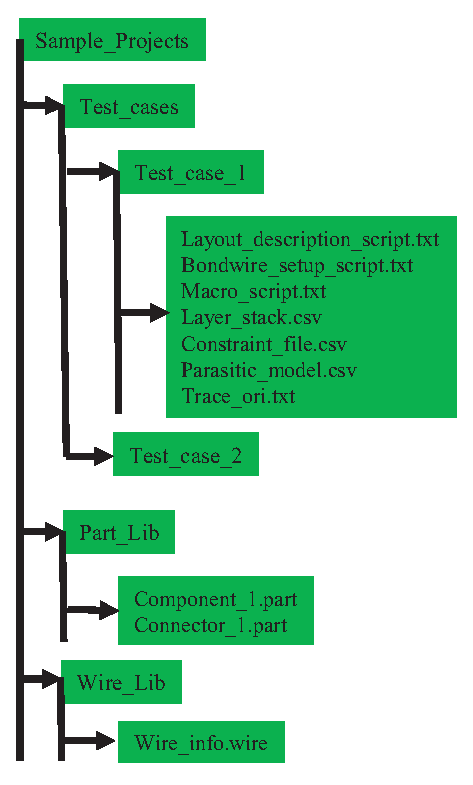
\includegraphics[width=3.5 in, height=5.8 in ]{figs/v_1.9_figs/folder_org.eps}
    \caption{Folder organization for PowerSynth v1.9 sample projects}
    \label{folder_org}
    \end{figure}

\pagebreak

\subsection{Walk-Through an Example}
    
A sample 2D half-bridge power module layout (shown in Figure~\ref{init_layout} (a)) is chosen for demonstrating the features of PowerSynth v1.9. To optimize the power loop inductance from DC+-to-DC- and maximum temperature of the layout, the layout script needs to be generated. Also, to represent the layout we need to have the following parts:\\
1. MOSFET, 2. Power Lead, 3. Signal Lead. The steps are described as follows:
\begin{enumerate}
    \item Prepare all part files and save in \textbf{Part\_Lib} folder. So, this folder should have:\\
    1. MOSFET.part
    2. Power\_Lead.part
    3. Signal\_Lead.part
    
    \item Create layout script. To represent the layout shown in Figure~\ref{init_layout}, the initial \textbf{Layout\_script} is shown in Listing~\ref{input_script}. Please note that all connected bond wire pads need to be aligned (i.e., horizontally or vertically) according to bottom-left coordinate of the pad.
    
    \begin{figure}[H]
    \centering
    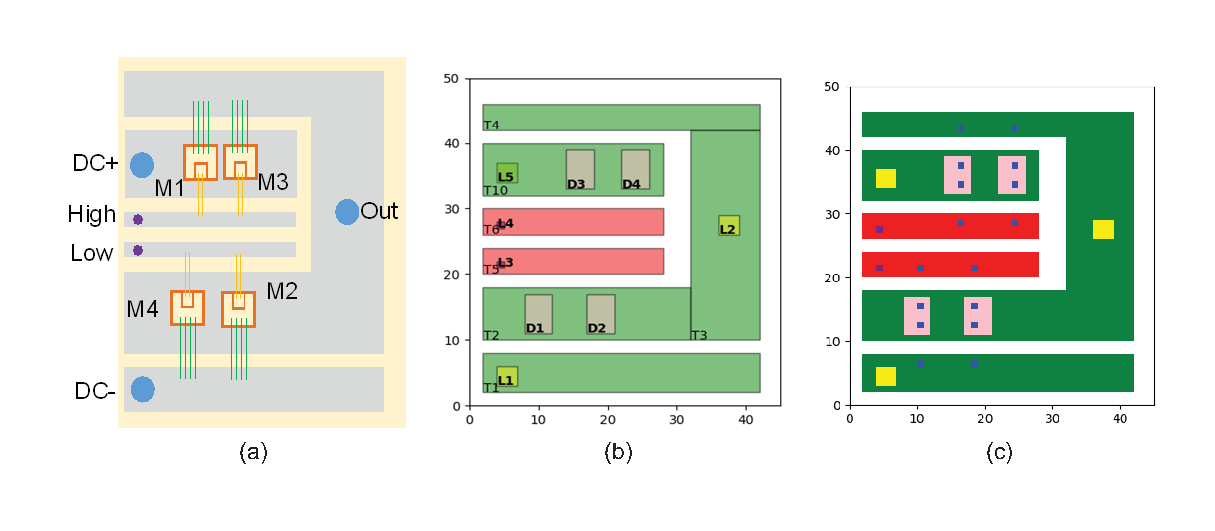
\includegraphics[width=\linewidth ]{figs/v_1.9_figs/Fig_example_layout.eps}
    \caption{(a) A sample half-bridge power module layout, (b) input layout without bonding wire pads, (c) script-generated layout}
    \label{init_layout}
    \end{figure}
    

    \pagebreak
    \begin{lstlisting} [caption={Layout\_script for the layout shown in Fig.~\ref{init_layout}},label={input_script}]
    
    # Definition
    power_lead ../../Part_Lib/power_lead.part
    signal_lead ../../Part_Lib/signal_lead.part
    MOS ../../Part_Lib/MOSFET.part
    
    #Layout Information
    45 50
    + T1 power 2 2 40 6 4
    	+ B1 power 10 6 1 1 5
    	+ B2 power 18 6 1 1 5
    	+ L1 power_lead 4 3 5
    + T2 power 2 10 30 8 4
    - T3 power 32 10 10 32 4
    - T4 power 2 42 40 4 4
    	+ B3 power 16 43 1 1 5
    	+ B4 power 24 43 1 1 5
    	+ L2 power_lead 36 26 5
    	+ D1 MOS 8 11 5
    		+ B5 signal 10 15 1 1 5
    		+ B6 power 10 12 1 1 5
    	+ D2 MOS 17 11 5
    		+ B7 signal 18 15 1 1 5
    		+ B8 power 18 12 1 1 5
    + T5 signal 2 20 26 4 4
    	+ B9 signal 10 21 1 1 5
    	+ B10 signal 18 21 1 1 5
    	+ L3 signal_lead 4 21 5
    + T6 signal 2 26 26 4 4
    	+ B11 signal 16 28 1 1 5
    	+ B12 signal 24 28 1 1 5
    	+ L4 signal_lead 4 27 5
    + T10 power 2 32 26 8 4
    	+ L5 power_lead 4 34 5
    	+ D3 MOS 14 33 5
    		+ B13 power 16 37 1 1 5
    		+ B14 signal 16 34 1 1 5
    	+ D4 MOS 22 33 5
    		+ B15 power 24 37 1 1 5
    		+ B16 signal 24 34 1 1 5

    
    \end{lstlisting}
    
    
    
    
    \item Prepare bond wire information file (*.wire) and save in \textbf{Wire\_Lib} directory. Sample file is provided in the \textbf{'Sample\_Projects-> Wire\_Lib}.
    
    \item Prepare bond wire connection definition script. The script content for this example case is shown in Listing~\ref{bondwire_script}.
    
    \begin{lstlisting} [caption={Bondwire\_setup file content},label={bondwire_script}]
    # Definition
    Wire1 ..\..\Wire_Lib\bond_wire_info.wire
    
    # Table_info
    BW1 Wire1 D1_Gate_B5 B9 1 0.1
    BW2 Wire1 D2_Gate_B7 B10 1 0.1
    BW3 Wire1 D1_Source_B6 B1 1 0.1
    BW4 Wire1 D2_Source_B8 B2 1 0.1
    BW5 Wire1 D3_Source_B13 B3 1 0.1
    BW6 Wire1 D4_Source_B15 B4 1 0.1
    BW7 Wire1 D3_Gate_B14 B11 1 0.1
    BW8 Wire1 D4_Gate_B16 B12 1 0.1

    \end{lstlisting}
    
    \item Prepare layer stack file and save as .csv format. The file content for this design is shown in Table~\ref{layer_stack}.
    \iffalse
    \begin{figure}[H]
    \centering
    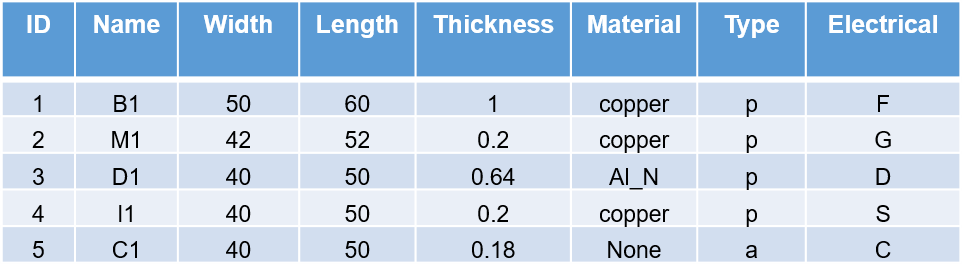
\includegraphics[width=6 in ]{figs/v_1.9_figs/Fig_140.PNG}
    \caption{Layer\_stack file content}
    \label{layer_stack}
    \end{figure}
    \fi
    
    \begin{table}[H]
      \centering
      \caption{Layer\_stack file content}
    \begin{tabular}{|c|c|c|c|c|c|c|c|}
    \hline
    ID    & Name  & Width & Length & Thickness & Material & Type  & Electrical \bigstrut\\
    \hline
    1     & B1    & 50    & 60    & 1     & copper & p     & F \bigstrut\\
    \hline
    2     & M1    & 42    & 52    & 0.2   & copper & p     & G \bigstrut\\
    \hline
    3     & D1    & 40    & 50    & 0.64  & Al\_N & p     & D \bigstrut\\
    \hline
    4     & I1    & 40    & 50    & 0.2   & copper & p     & S \bigstrut\\
    \hline
    5     & C1    & 40    & 50    & 0.18  & None  & a     & C \bigstrut\\
    \hline
    \end{tabular}%
  \label{layer_stack}%
\end{table}%
    
    
    \item Create a blank csv file for constraints. For this case, the file name is "layout.csv". 
    
    \item Prepare the trace orientation file. The content for this design is shown in Listing~\ref{trace_ori}
    \iffalse
    \begin{figure}[H]
    \centering
    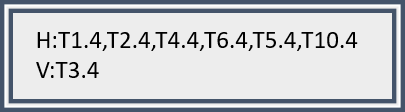
\includegraphics[width=3 in ]{figs/v_1.9_figs/Fig_240.PNG}
    \caption{Trace\_Ori file content}
    \label{trace_ori}
    \end{figure}
    \fi
    
    \begin{lstlisting} [caption={Trace\_Ori file content},label={trace_ori}]
    H:T1.4,T2.4,T4.4,T6.4,T5.4,T10.4
    V:T3.4

    
    \end{lstlisting}
    
    \item Populate all paths in the fields of the \textbf{`\#Input\_scripts:'} in the macro script. At this stage the macro script would look like Listing~\ref{macro_1}.
    \pagebreak
    \iffalse
    \begin{figure}[H]
    \centering
    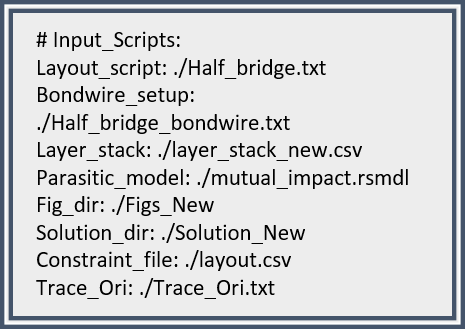
\includegraphics[width=4 in ]{figs/v_1.9_figs/Fig_150.PNG}
    \caption{Macro script with input files content}
    \label{macro_1}
    \end{figure}   
    \fi
    
    \begin{lstlisting} [caption={Macro script with input files content},label={macro_1}]
    # Input_Scripts:
    Layout_script: ./Half_bridge.txt
    Bondwire_setup: ./Half_bridge_bondwire.txt
    Layer_stack: ./layer_stack_new.csv
    Parasitic_model: ./mutual_impact.rsmdl
    Fig_dir: ./Figs_New
    Solution_dir: ./Solution_New
    Constraint_file: ./layout.csv
    Trace_Ori: ./Trace_Ori.txt

    \end{lstlisting}
    
    \item Set up parameters for layout optimization according to layout solution evaluation mode. For example, we want to apply reliability constraints and optimize a fixed-sized layout with size of (45× 55). The macro script content is shown in Listing~\ref{macro_2}.
    \iffalse
    \begin{figure}[H]
    \centering
    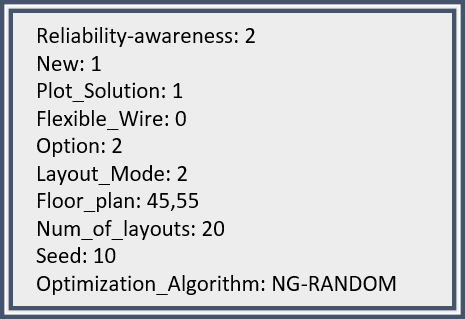
\includegraphics[width=3.8 in ]{figs/v_1.9_figs/Fig_160.PNG}
    \caption{Fixed-sized solutions parameters}
    \label{macro_2}
    \end{figure} 
    \fi
    \begin{lstlisting} [caption={Layout generation setup parameters for fixed-sized optimization},label={macro_2}]
    Reliability-awareness: 2
    New: 1
    Plot_Solution: 1
    Flexible_Wire: 0
    Option: 2
    Layout_Mode: 2
    Floor_plan: 45,55 
    Num_of_layouts: 20
    Seed: 10
    Optimization_Algorithm: NG-RANDOM

    \end{lstlisting}
    
    \item Setup performance metrics. For electro-thermal optimization, the electrical, and thermal setup content are shown in Listing~\ref{macro_3}, Listing~\ref{macro_4}, respectively.
    \iffalse
    \begin{figure}[H]
    \centering
    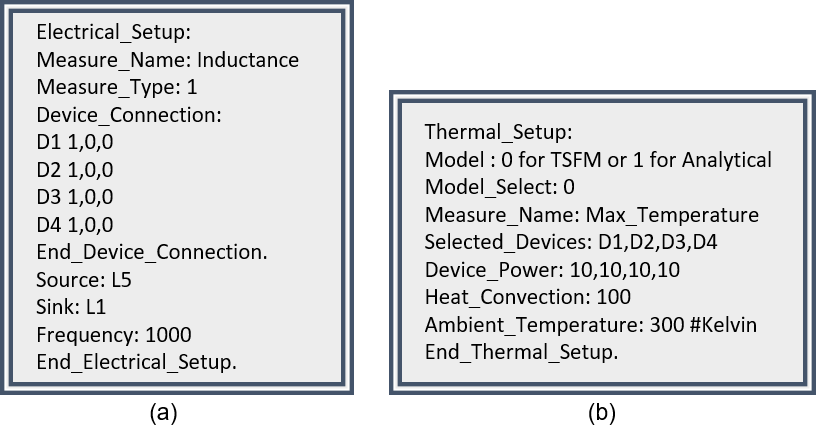
\includegraphics[width=\linewidth ]{figs/v_1.9_figs/Fig_170.PNG}
    \caption{(a) Electrical performance setup, (b) thermal performance setup}
    \label{macro_3}
    \end{figure}  
    \fi
    \begin{lstlisting} [caption={Electrical performance evaluation parameters setup},label={macro_3}]
   Electrical_Setup:
    Measure_Name: Inductance
    Measure_Type: 1
    Device_Connection:
    D1 1,0,0
    D2 1,0,0
    D3 1,0,0
    D4 1,0,0
    End_Device_Connection.
    Source: L5
    Sink: L1
    Frequency: 1000
    End_Electrical_Setup.
    \end{lstlisting}
    \pagebreak
    \begin{lstlisting} [caption={Thermal performance evaluation parameters setup},label={macro_4}]
    Thermal_Setup:
    # Model : 0 for TSFM or 1 for Analytical
    Model_Select: 0
    Measure_Name: Max_Temperature
    Selected_Devices: D1,D2,D3,D4
    Device_Power: 10,10,10,10
    Heat_Convection: 100
    Ambient_Temperature: 300
    End_Thermal_Setup.

    
    \end{lstlisting}
    
    \iffalse
    \begin{figure}[t]
    \centering
    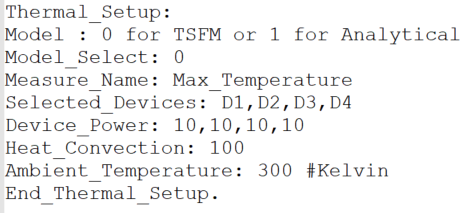
\includegraphics[width=\linewidth ]{figs/v_1.9_figs/Fig_18.PNG}
    \caption{Thermal performance setup}
    \label{macro_4}
    \end{figure} 
    \fi
    
    \item Run \textbf{"PowerSynth.exe"}. In command prompt it will appear as shown in Figure~\ref{macro_5}.
    
    \begin{figure}[H]
    \centering
    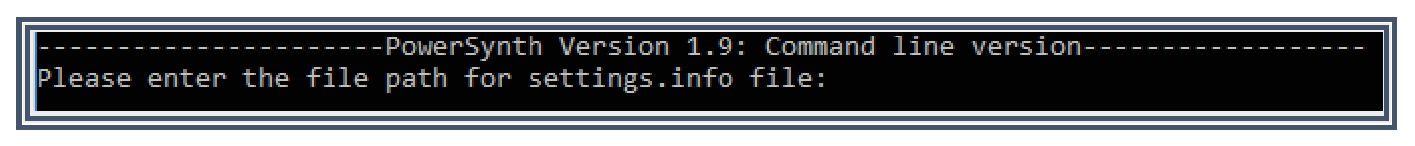
\includegraphics[width=\linewidth ]{figs/v_1.9_figs/cmd_re_1.eps}
    \caption{Running PowerSynth}
    \label{macro_5}
    \end{figure} 
    
    \item Now provide the path of your \textbf{"settings.info"} file location. This sample file is provided in the package. You can modify the individual file path according to your environment. The settings file content is shown in Listing~\ref{settings}.
    \iffalse
    \begin{figure}[H]
    \centering
    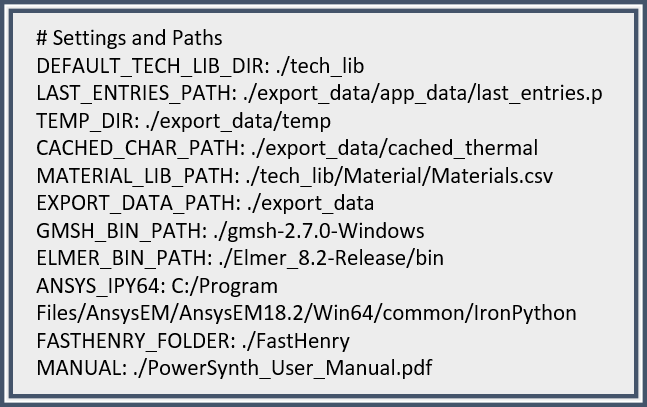
\includegraphics[width=5 in ]{figs/v_1.9_figs/Fig_200.PNG}
    \caption{Settings file content}
    \label{settings}
    \end{figure}
    \fi
    
    \begin{lstlisting} [caption={Settings file content},label={settings}]
    # Settings and Paths
    DEFAULT_TECH_LIB_DIR: ./tech_lib
    LAST_ENTRIES_PATH: ./export_data/app_data/last_entries.p
    TEMP_DIR: ./export_data/temp
    CACHED_CHAR_PATH: ./export_data/cached_thermal
    MATERIAL_LIB_PATH: ./tech_lib/Material/Materials.csv
    EXPORT_DATA_PATH: ./export_data
    GMSH_BIN_PATH: ./gmsh-2.7.0-Windows
    ELMER_BIN_PATH: ./Elmer_8.2-Release/bin
    ANSYS_IPY64: C:/Program Files/AnsysEM/../../../IronPython
    FASTHENRY_FOLDER: ./FastHenry
    MANUAL: ./PowerSynth_User_Manual.pdf

    \end{lstlisting}
    
    \item Upon entering the file info it will ask for \textbf{Macro script"} location. After providing that, the command prompt would be similar as Figure~\ref{macro_6}.
    
    \begin{figure}[H]
    \centering
    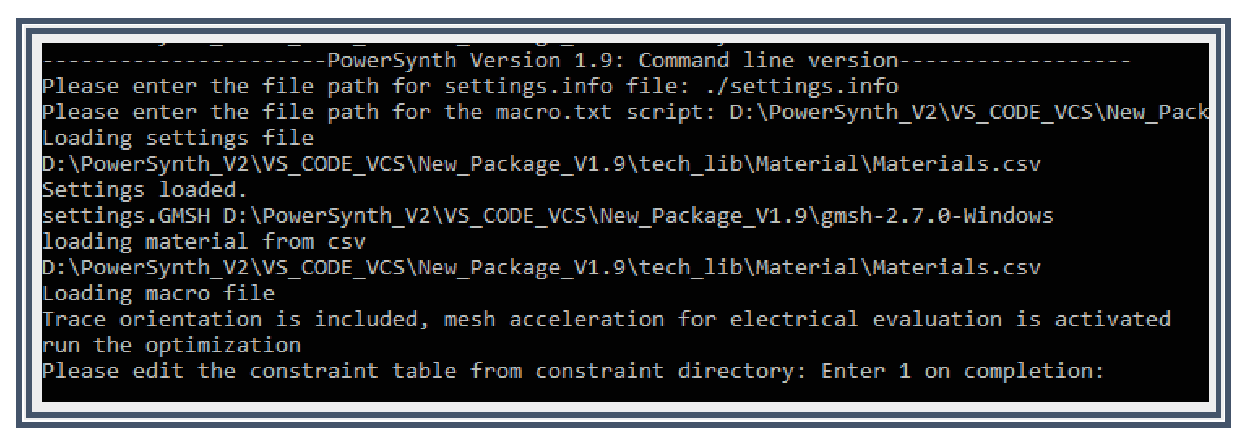
\includegraphics[width=\linewidth ]{figs/v_1.9_figs/cmd_re_2.eps}
    \caption{Running PowerSynth (ctd)}
    \label{macro_6}
    \end{figure}
    
    Since we have set up \textbf{New} flag as 1, it is asking user to edit constraint table. The initial table looks like as shown in Figure~\ref{cons_init}. For this example, the DC+ voltage is 15 KV, and DC- is 0V. The expected AC voltage is a sinusoid with min and max amplitude is 0 V, 15 KV, respectively and the frequency is 10 KHz. For the gate signal, the voltage is switching in between -5V and 20V with very high switching frequency (1 MHz). For power traces, and gate traces, the current loading is assumed to be 15A, and 20 mA, respectively.
    So, these information should be provided in the proper waveform format as discussed in Section~\ref{sec-2-2-1} (\textbf{Constraints}). 
    After editing the table and providing all constraint information, the table looks like the one as shown in Fig.~\ref{cons_up}. Please note that, the voltage difference column has a constant difference of 5000 V and the current rating column has a constant increment of 5 A.
    \begin{figure}[H]
    \centering
    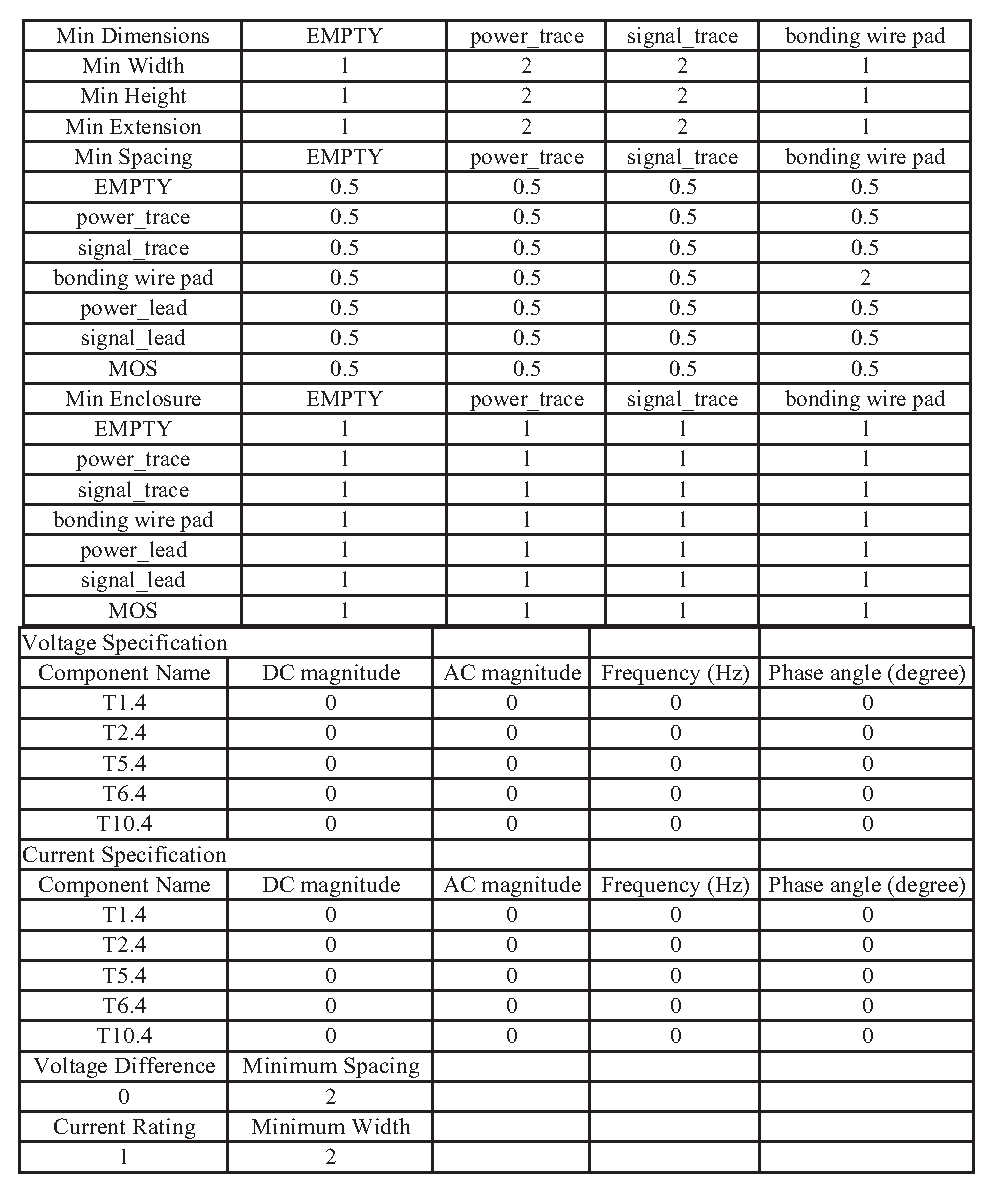
\includegraphics[width=\linewidth ]{figs/v_1.9_figs/Cons_init.eps}
    \caption{Constraint table content}
    \label{cons_init}
    \end{figure}
    
    \begin{figure}[H]
    \centering
    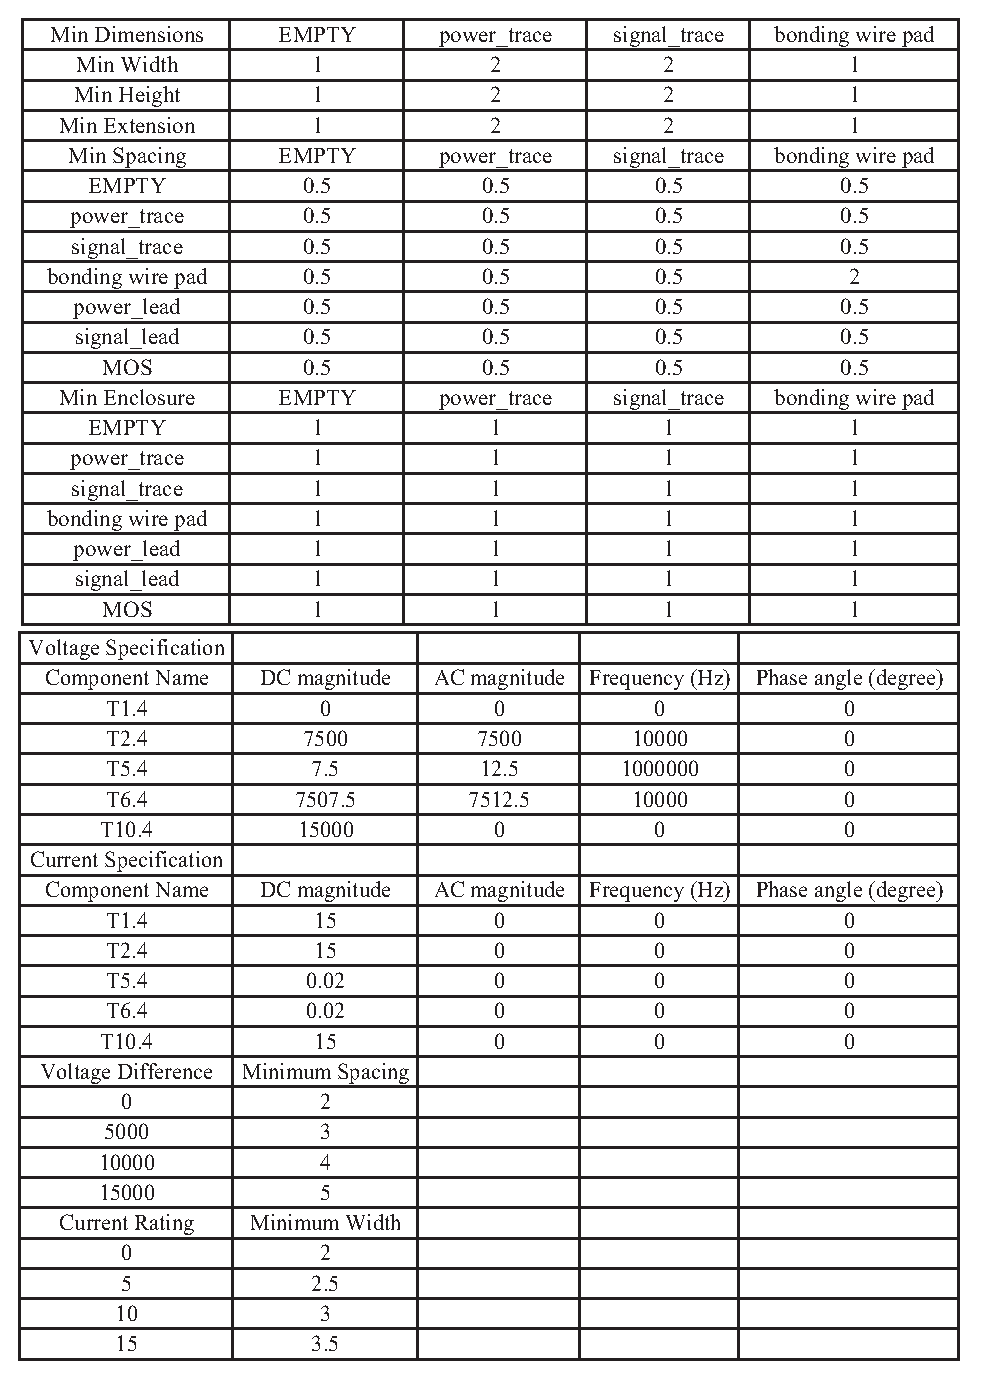
\includegraphics[width=\linewidth, height=8.5 in ]{figs/v_1.9_figs/cmd_re_4.eps}
    \caption{Constraint table content after update}
    \label{cons_up}
    \end{figure}    
    Once editing the constraint table, enter 1 in the command line.
    Then it will generate 20 solutions and several files will be saved in “Solution\_dir” and “Fig\_dir”. Results can be found in "Sample\_Projects/Test\_Cases/Half\_Bridge\_2" folder in the package.
    
    For large number of solutions, we should turn off “Plot\_Solutions” flag, otherwise you may encounter “memory” issue in python.
    To use the updated constraint table, user should turn off the “New” flag, otherwise each time user runs PowerSynth.exe with the same macro script, it asks for editing constraint table and overwrite the modified values with the default values.
    By changing “Option”, “Layout\_Mode”, user can use PowerSynth according to the necessity.

    

\end{enumerate}









\section{PowerSynth-Related Publications}


This section contains a list of all the current publications related to PowerSynth as of the date of this document.

\begin{enumerate}
\item P. Tucker, "\href{./Publications/TUCKER-THESIS.pdf}{SPICE netlist generation for electrical parasitic modeling of multi-chip power module designs}," 2013.

\item B. W. Shook, A. Nizam, Z. Gong, A. M. Francis and H. A. Mantooth, "\href{./Publications/COMPEL paper.pdf}{Multi-objective layout optimization for multi-chip power modules considering electrical parasitics and thermal performance}," in \emph{Control and Modeling for Power Electronics (COMPEL)}, \emph{2013 IEEE 14th Workshop on}, 2013.

\item B. W. Shook, Z. Gong, Y. Feng, A. M. Francis and H. A. Mantooth, "\href{./Publications/CAD_9_6__837-846.pdf}{Multi-chip power module fast thermal modeling for layout optimization}," \emph{Computer-Aided Design and Applications}, vol. 9, pp. 837-846, 2012.

\item B. W. Shook, "\href{./Publications/Shook_Brett_thesis.pdf}{The Design and Implementation of a Multi-Chip Power Module Layout Synthesis Tool}," 2014.

\item J. Main, "\href{./Publications/Jonathan_Main_Thesis.pdf}{A Manufacturer Design Kit for Multi-Chip Power Module Layout Synthesis}," 2017.

\item Q. Le, T. Evans, S. Mukherjee, Y. Peng, T. Vrotsos and H. A. Mantooth, "\href{./Publications/WIPDA 2017.pdf}{Response surface modeling for parasitic extraction for multi-objective optimization of multi-chip power modules (MCPMs)}," \emph{in Wide Bandgap Power Devices and Applications (WiPDA)}, \emph{2017 IEEE 5th Workshop on}, 2017.

\item Q. Le, S. Mukherjee, T. Vrotsos and H. A. Mantooth, "\href{./Publications/COMPEL_2016_paper_140.pdf}{Fast transient thermal and power dissipation modeling for multi-chip power modules: A preliminary assessment of different electro-thermal evaluation methods}," in \emph{Control and Modeling for Power Electronics (COMPEL)}, \emph{2016 IEEE 17th Workshop on}, 2016.

\item Z. Gong, "\href{./Publications/Gong_Zihao_thesis.pdf}{Thermal and electrical parasitic modeling for multi-chip power module layout synthesis}," 2012.



\item S. Mukherjee et al, "\href{./Publications/PID5441927.pdf}{Toward Partial Discharge Reduction by Corner Correction in Power Module Layouts}," in \emph{Control and Modeling for Power Electronics (COMPEL)},  pp. 1–8, Jun 2018.


\item I. Al Razi et al, "\href{./Publications/WIPDA_2018.pdf}{Constraint-Aware Algorithms for Heterogeneous Power Module Layout Synthesis and Reliability Optimization}," in \emph{ Wide Bandgap Power Devices and Applications (WiPDA)}, pp. 323–330, Oct 2018.

\item T. Evans, Q. Le, S. Mukherjee, I. Al Razi, T. Vrotsos, Y. Peng and H. A. Mantooth, "\href{./Publications/PowerSynth-A_Module_Layout_Generation_Tool.pdf}{PowerSynth: A Module Layout Generation Tool}," in \emph{IEEE Transactions on Power Electronics}, vol. 34, no. 6, pp. 5063–5078, Jun 2019, Highlighted Paper.


\item Q. Le et al, "\href{./Publications/Q.Le_IWIPP_19.pdf}{PEEC Method and Hierarchical Approach Towards 3D Multichip Power Module (MCPM) Layout Optimization}", in Proc. IEEE International Workshop on Integrated Power Packaging, pp. 131–136, Apr 2019.

\item 	I. Al Razi et al, "\href{./Publications/I.Al.Razi-ECCE_19.pdf} {Hierarchical Layout Synthesis and Design Automation for 2.5D Heterogeneous Multi-Chip Power Modules}", in Proc. IEEE Energy Conversion Congress and Exposition, pp. 2257-2263, Sep 2019.

\item T. Evans et al, "\href{./Publications/T.Evans_IMAPS_19.pdf}{Development of EDA Techniques for Power Module EMI Modeling and Layout Optimization}", in Proc. IMAPS International Symposium on Microelectronics, pp. 193-198, Oct 2019.

\item Y. Peng et al, "\href{./Publications/Y.Peng_NOLTA_20.pdf}{PowerSynth Progression on Layout Optimization for Reliability and Signal Integrity}", IEICE Nonlinear Theory and Its Applications, vol. 11, no. 2, pp. 124-144, Apr 2020, Invited Paper.

\item 	I. Al Razi et al, "\href{./Publications/I.Al.Razi-ECCE_20.pdf}{Physical Design Automation for High-Density 3D Power Module Layout Synthesis and Optimization}", (accepted) in Proc. IEEE Energy Conversion Congress and Exposition, 2020.

\item T. Evans et al, "\href{./Publications/T.Evans-ECCE_20.pdf}{Electronic Design Automation Tools and Considerations for Electro-Thermo-Mechanical Co-Design of High Voltage Power Modules}", (accepted) in Proc. IEEE Energy Conversion Congress and Exposition, 2020.

\item 	S. Mukherjee et al, "\href{./Publications/S.Mukherjee_WiPDA-Asia_20.pdf}{General Equation to Determine Design Rules for Mitigating Partial Discharge and Electrical Breakdown in Power Module Layouts}", (accepted) in Proc. IEEE Workshop on Wide Bandgap Power Devices and Applications in Asia, 2020.
\end{enumerate}

\subsection{Useful Links}

\begin{itemize}
    \item \textbf{Release Website:} \href{https://e3da.csce.uark.edu/release/PowerSynth/}{\underline{https://e3da.csce.uark.edu/release/PowerSynth/}}
    \item \textbf{Publication Website:} \href{https://e3da.csce.uark.edu/pub/}{\underline{https://e3da.csce.uark.edu/pub/}}
\end{itemize}



\pagebreak

\section{Authors}
The PowerSynth tool development is on-going for a decade now and the current PowerSynth team appreciates efforts from quite a few number of graduate students and numerous undergraduate students over the years.
\subsection{Graduate Research Assistants}
The PowerSynth research and development team worked on this version (v1.9) consists of four Ph.D. students from different disciplines, who are supervised by two professors. A brief introduction to the authors are as follows:

\begin{itemize}

\item \textbf{Imam Al Razi} \\
Ph.D. Student\\
Computer Science and Computer Engineering Department\\
University of Arkansas, Fayetteville, AR, USA.


\item \textbf{Quang Le} \\
Ph.D. Student\\
Electrical Engineering Department\\
University of Arkansas, Fayetteville, AR, USA.\\


\item\textbf{Tristan M. Evans}\\
Ph.D. Student\\
Electrical Engineering Department\\
University of Arkansas, Fayetteville, AR, USA.\\

\item\textbf{Shilpi Mukherjee}\\
Ph.D. Student\\
Microelectronics and Photonics Department\\
University of Arkansas, Fayetteville, AR, USA.\\
\end{itemize}

\subsection{Supervisors}

\begin{itemize}
   
\item\textbf{Dr. Homer Alan Mantooth}\\
Distinguished Professor, The Twenty-First Century Research Leadership Chair in Engineering\\
Department of Electrical Engineering, University of Arkansas, Fayetteville, AR, USA.\\
Phone: 479-575-4838\\
Email: mantooth@uark.edu\\

\item\textbf{Dr. Yarui Peng}\\
Assistant Professor\\
Computer Science and Computer Engineering Department\\ 
University of Arkansas, Fayetteville, AR, USA.\\
Phone: 479-575-6043\\
Email: yrpeng@uark.edu\\  

\end{itemize}



% Emacs 25.2.1 (Org mode 8.2.10)
\end{document}



